\begin{appendices}

%%%%%%%%%%%%%%%%%%%%%%%%%%%%%%%%%%%%%%%%%%%%%%%%%%%%%%%%%%%%%%%%%%%%%%%%%%%%



\section{Impact du chlore} 
\label{appendix:chlore}
\subsection*{Traceurs atomiques}
\begin{figure}[!h]
    \centering 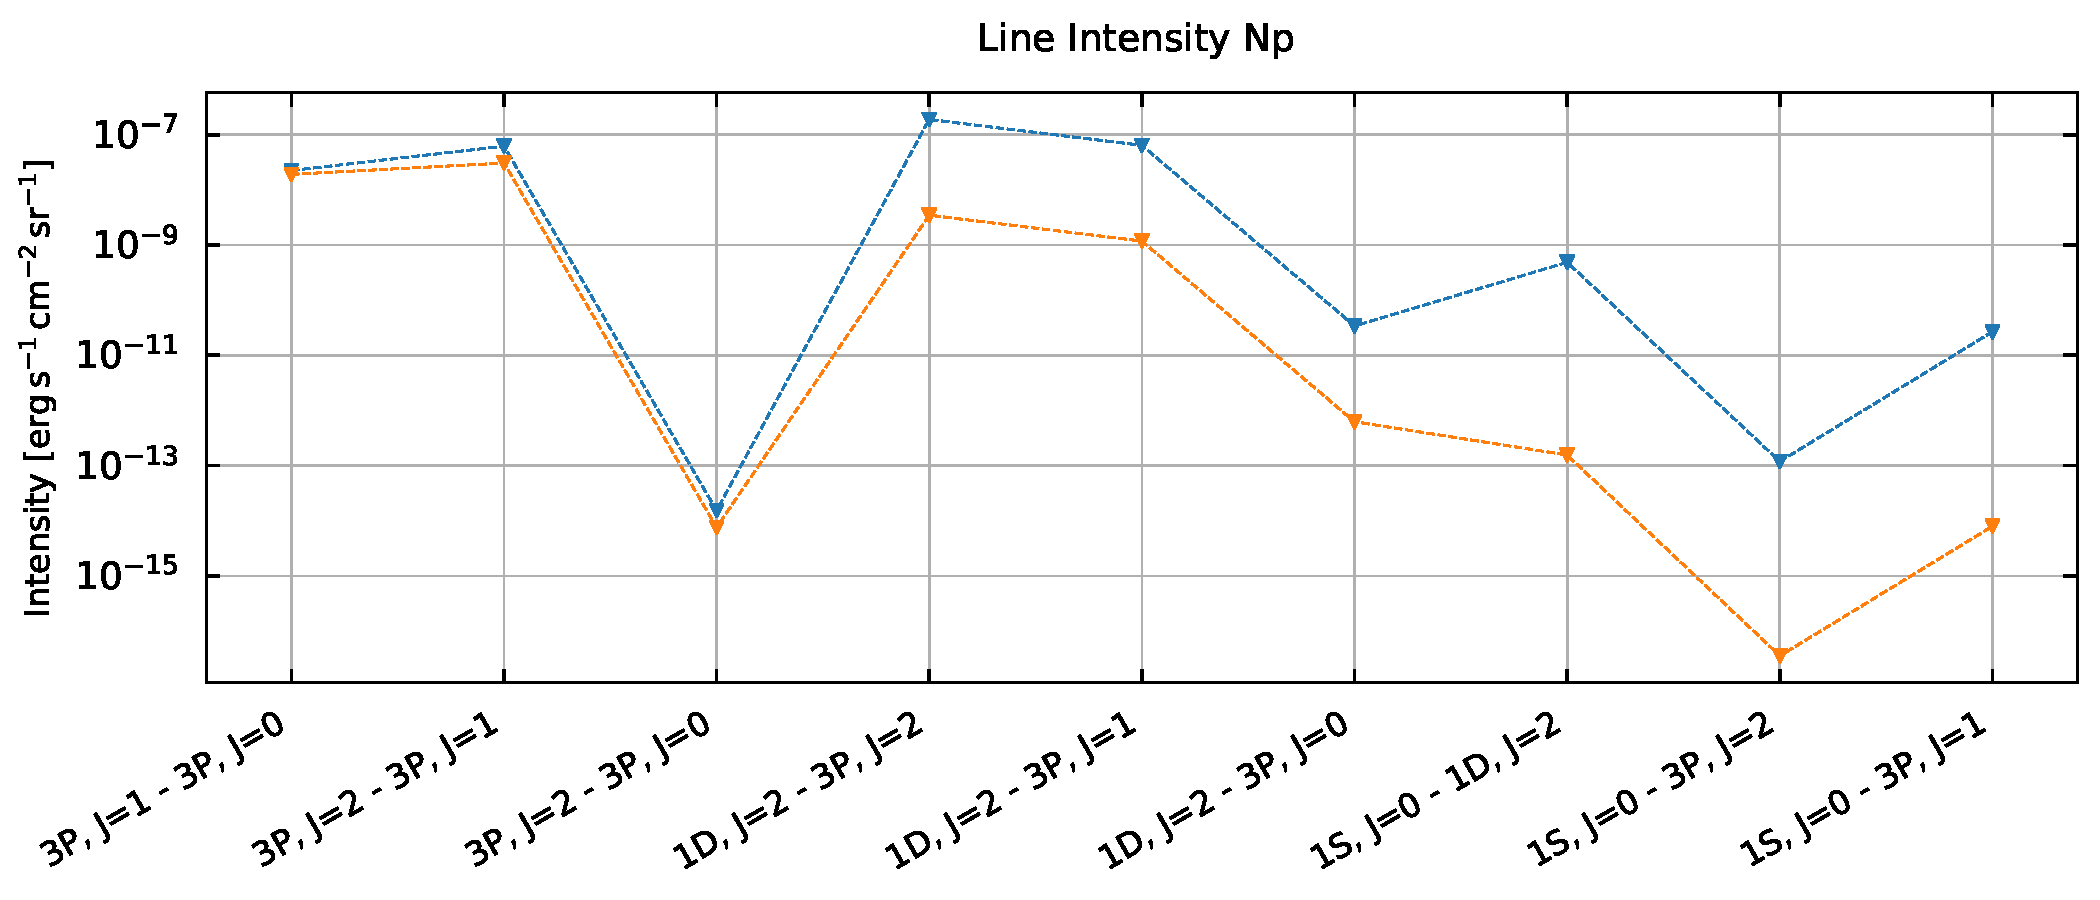
\includegraphics[trim = {0 0 0 1cm},clip,width=1\textwidth]{figure/Cl/gridModelEmiss/I_comp_Np.pdf}
        \caption{Diagramme d'intensité de $\mathrm{N}^+$}
        \label{fig:cl:emiss:Np}
\end{figure}

\begin{figure}[!h]
    \centering 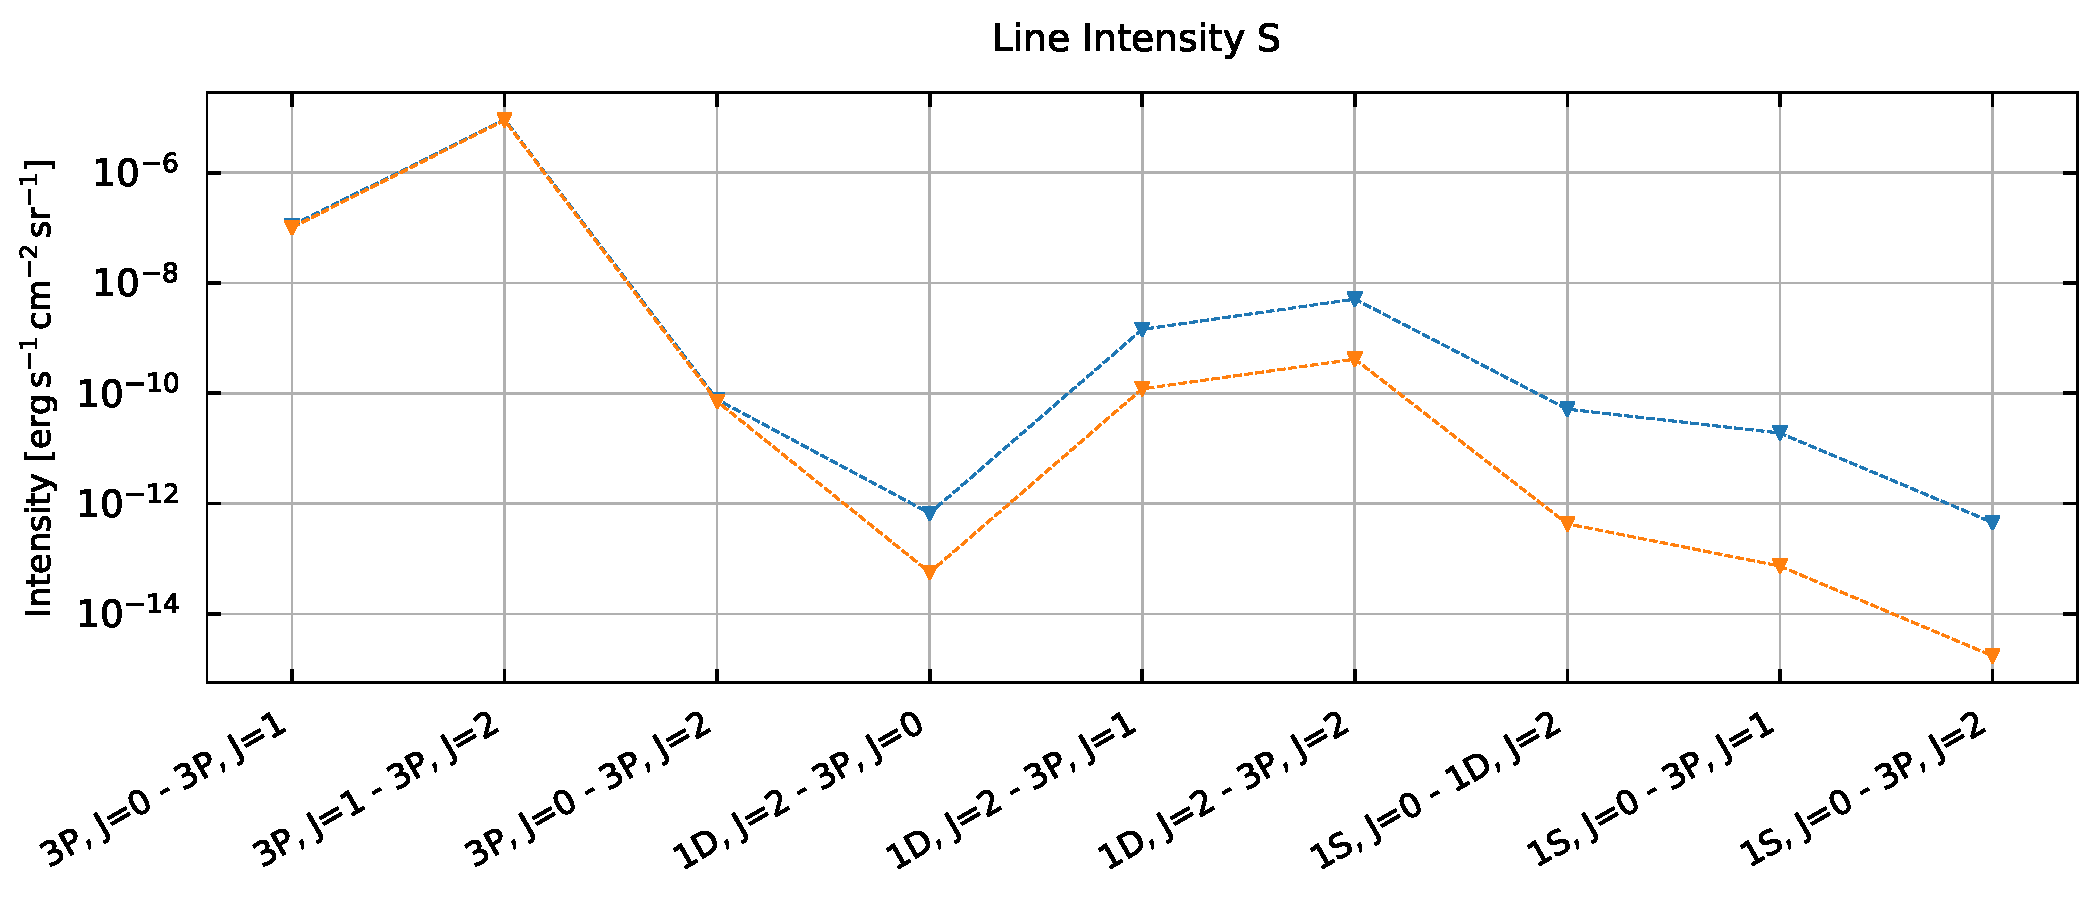
\includegraphics[trim = {0 0 0 1cm},clip,width=1\textwidth]{figure/Cl/gridModelEmiss/I_comp_S.pdf}
        \caption{Diagramme d'intensité de $\mathrm{S}$}
        \label{fig:cl:emiss:S}
\end{figure}

\begin{figure}[!h]
    \centering 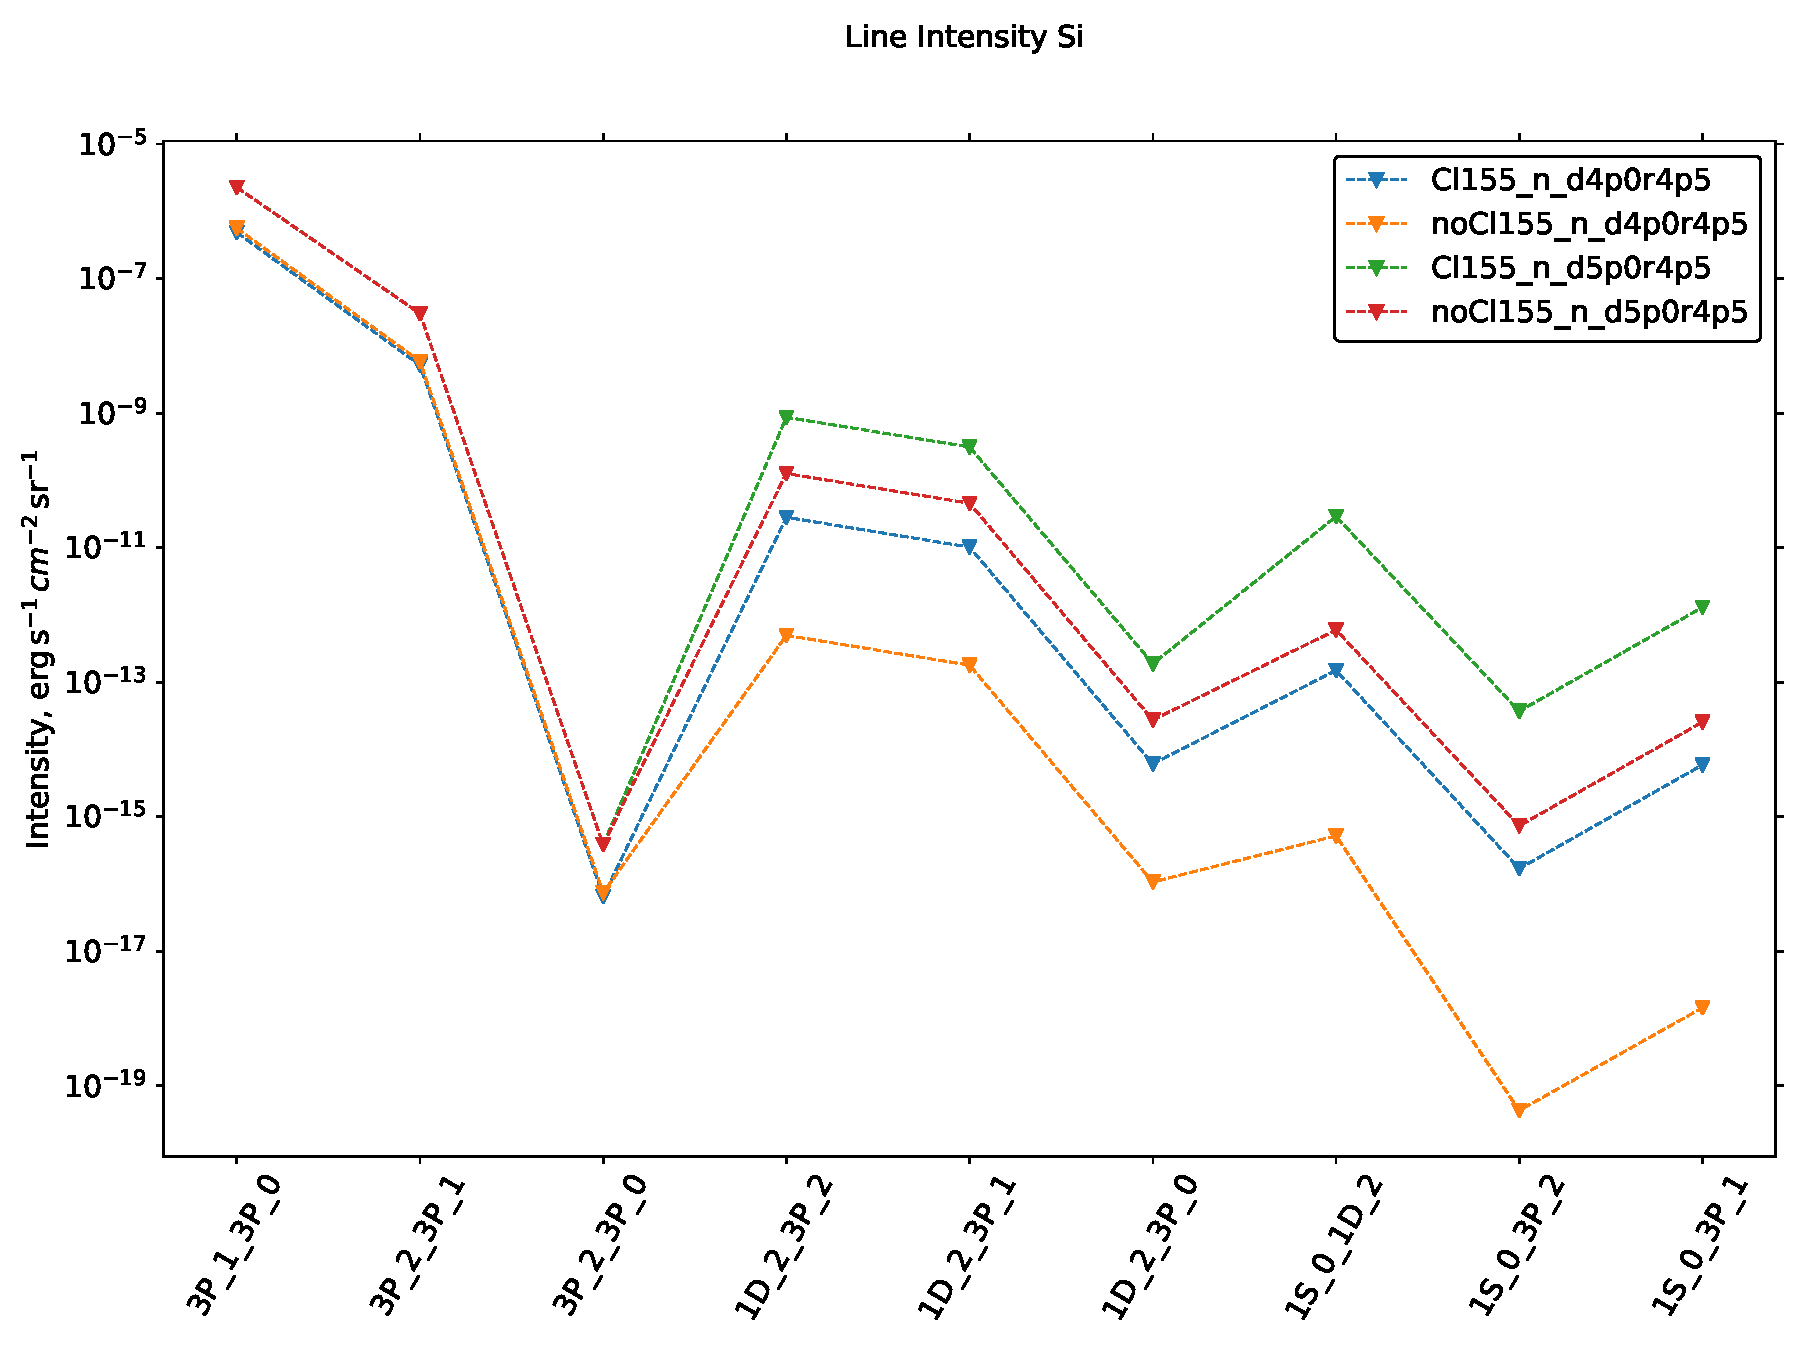
\includegraphics[trim = {0 0 0 1cm},clip,width=1\textwidth]{figure/Cl/gridModelEmiss/I_comp_Si.pdf}
        \caption{Diagramme d'intensité de $\mathrm{Si}$}
        \label{fig:cl:emiss:Si}
\end{figure}

\begin{figure}[!h]
    \centering
    \begin{subfigure}[t]{0.49\textwidth} % "0.49" donne ici la largeur de l'image
        \centering 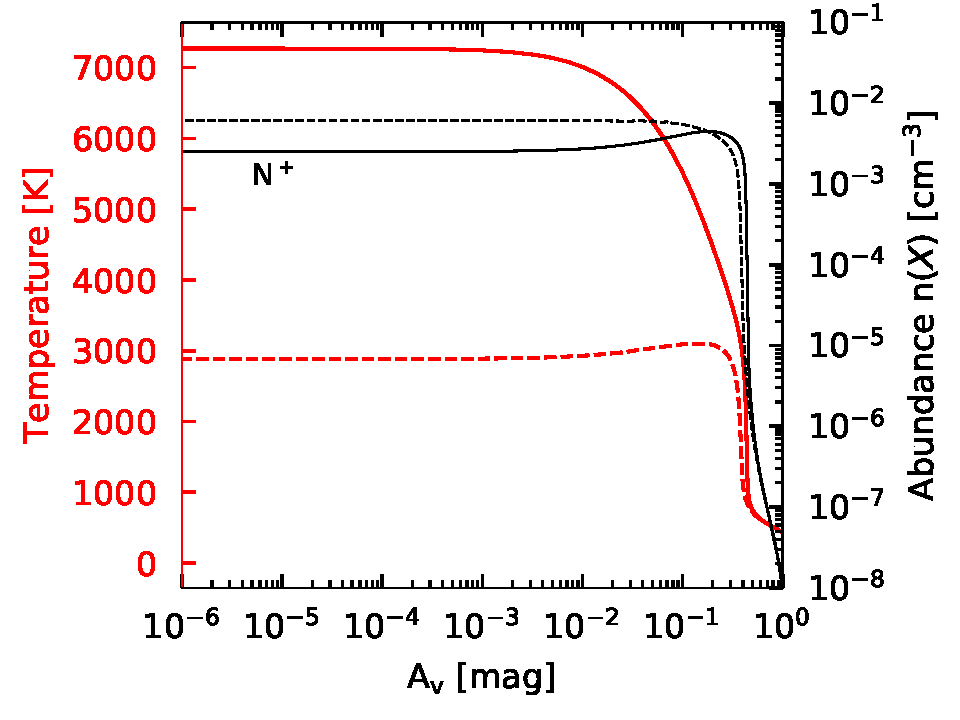
\includegraphics[trim = {0 0 0 0},clip,width=1\textwidth]{figure/Cl/gridModelEmiss/nT_comp_Np.pdf}
        \caption{$\mathrm{N}^+$}
    \end{subfigure}
    ~ 
   \begin{subfigure}[t]{0.49\textwidth} % "0.49" donne ici la largeur de l'image
        \centering 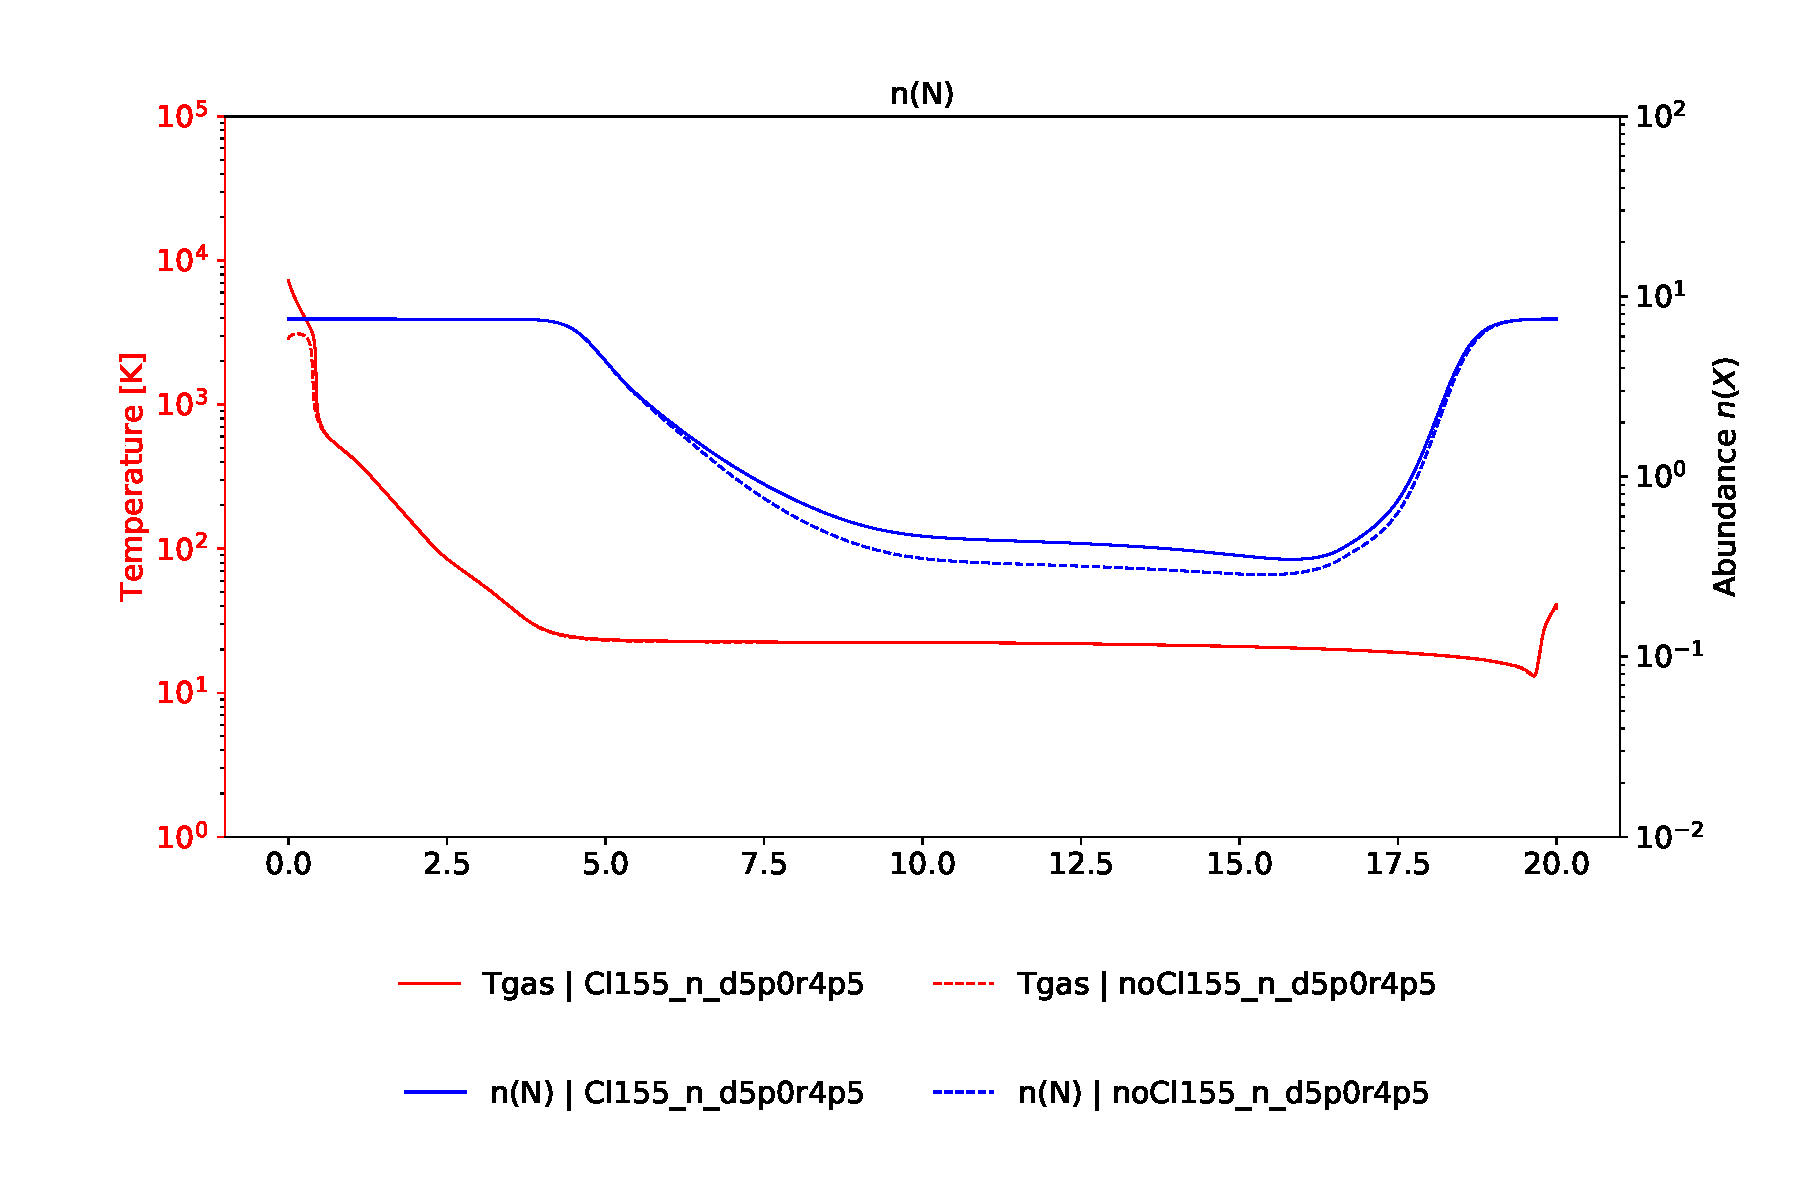
\includegraphics[trim = {0 0 0 0},clip,width=1\textwidth]{figure/Cl/gridModelEmiss/nT_comp_N.pdf}
        \caption{$\mathrm{N}$}
    \end{subfigure}
    
    \begin{subfigure}[t]{0.49\textwidth} % "0.49" donne ici la largeur de l'image
        \centering 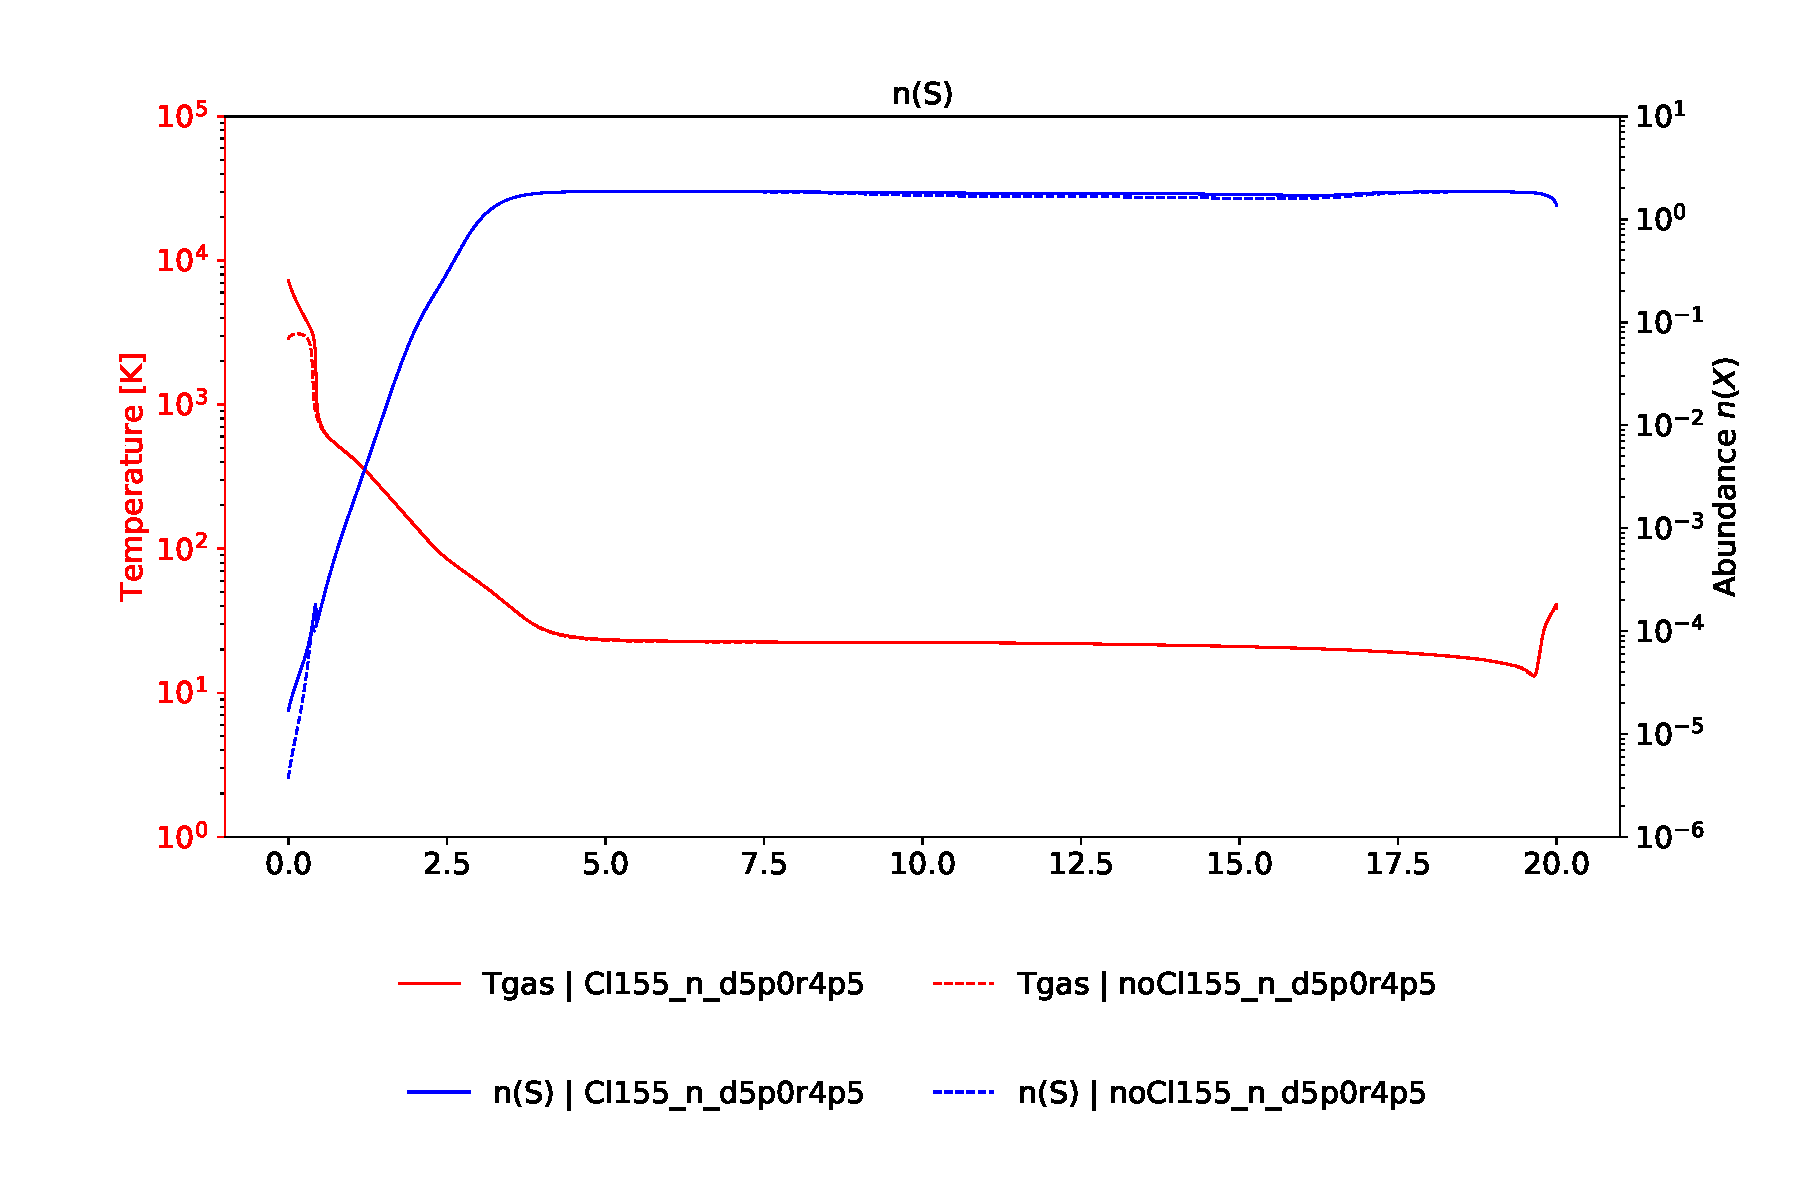
\includegraphics[trim = {0 0 0 0},clip,width=1\textwidth]{figure/Cl/gridModelEmiss/nT_comp_S.pdf}
        \caption{$\mathrm{S}$}
    \end{subfigure}
    ~
    \begin{subfigure}[t]{0.49\textwidth} % "0.49" donne ici la largeur de l'image
        \centering 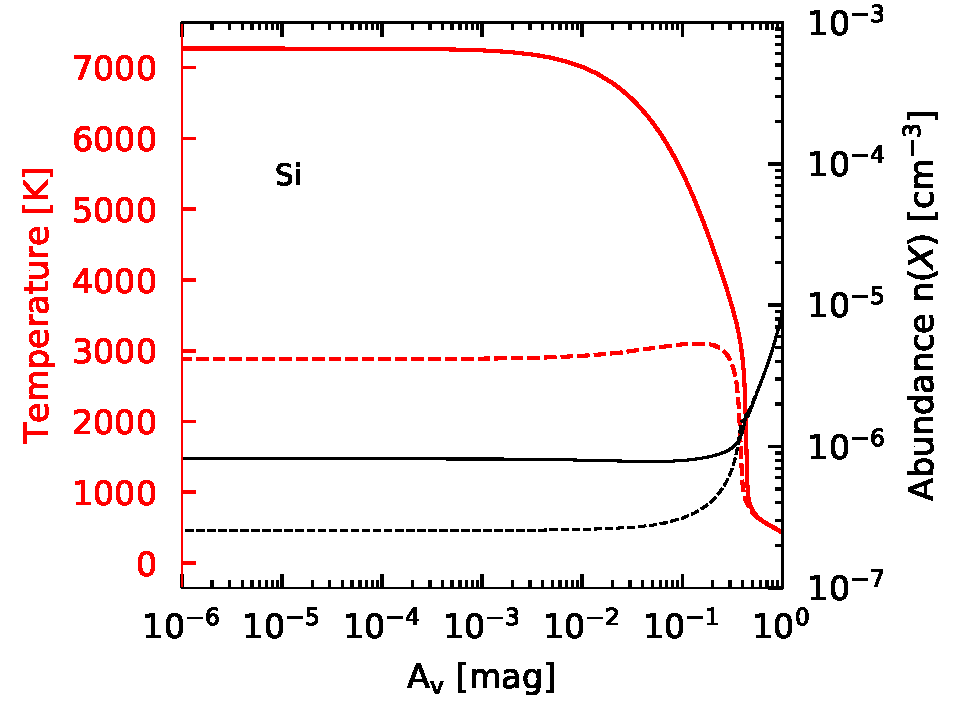
\includegraphics[trim = {0 0 0 0},clip,width=1\textwidth]{figure/Cl/gridModelEmiss/nT_comp_Si.pdf}
        \caption{$\mathrm{Si}$}
    \end{subfigure}
    
    \caption{Profils de densité des traceurs impactés par l'ajout du chlore.}
    \begin{minipage}{\textwidth}
    Il est représenté en trait plein les profils du modèle avec le chlore et en trait pointillé le modèle ne contenant pas de chlore. La température est en rouge et la densité en noir. On constate que l'augmentation de la température induite par le chlore facilite la formation des traceurs atomiques. 
    \end{minipage}
    \label{fig:Cl:gridModelEmiss:nT:yes}
\end{figure}

\clearpage
\subsection*{Traceurs moléculaires}


\begin{figure}[!h]
        \centering 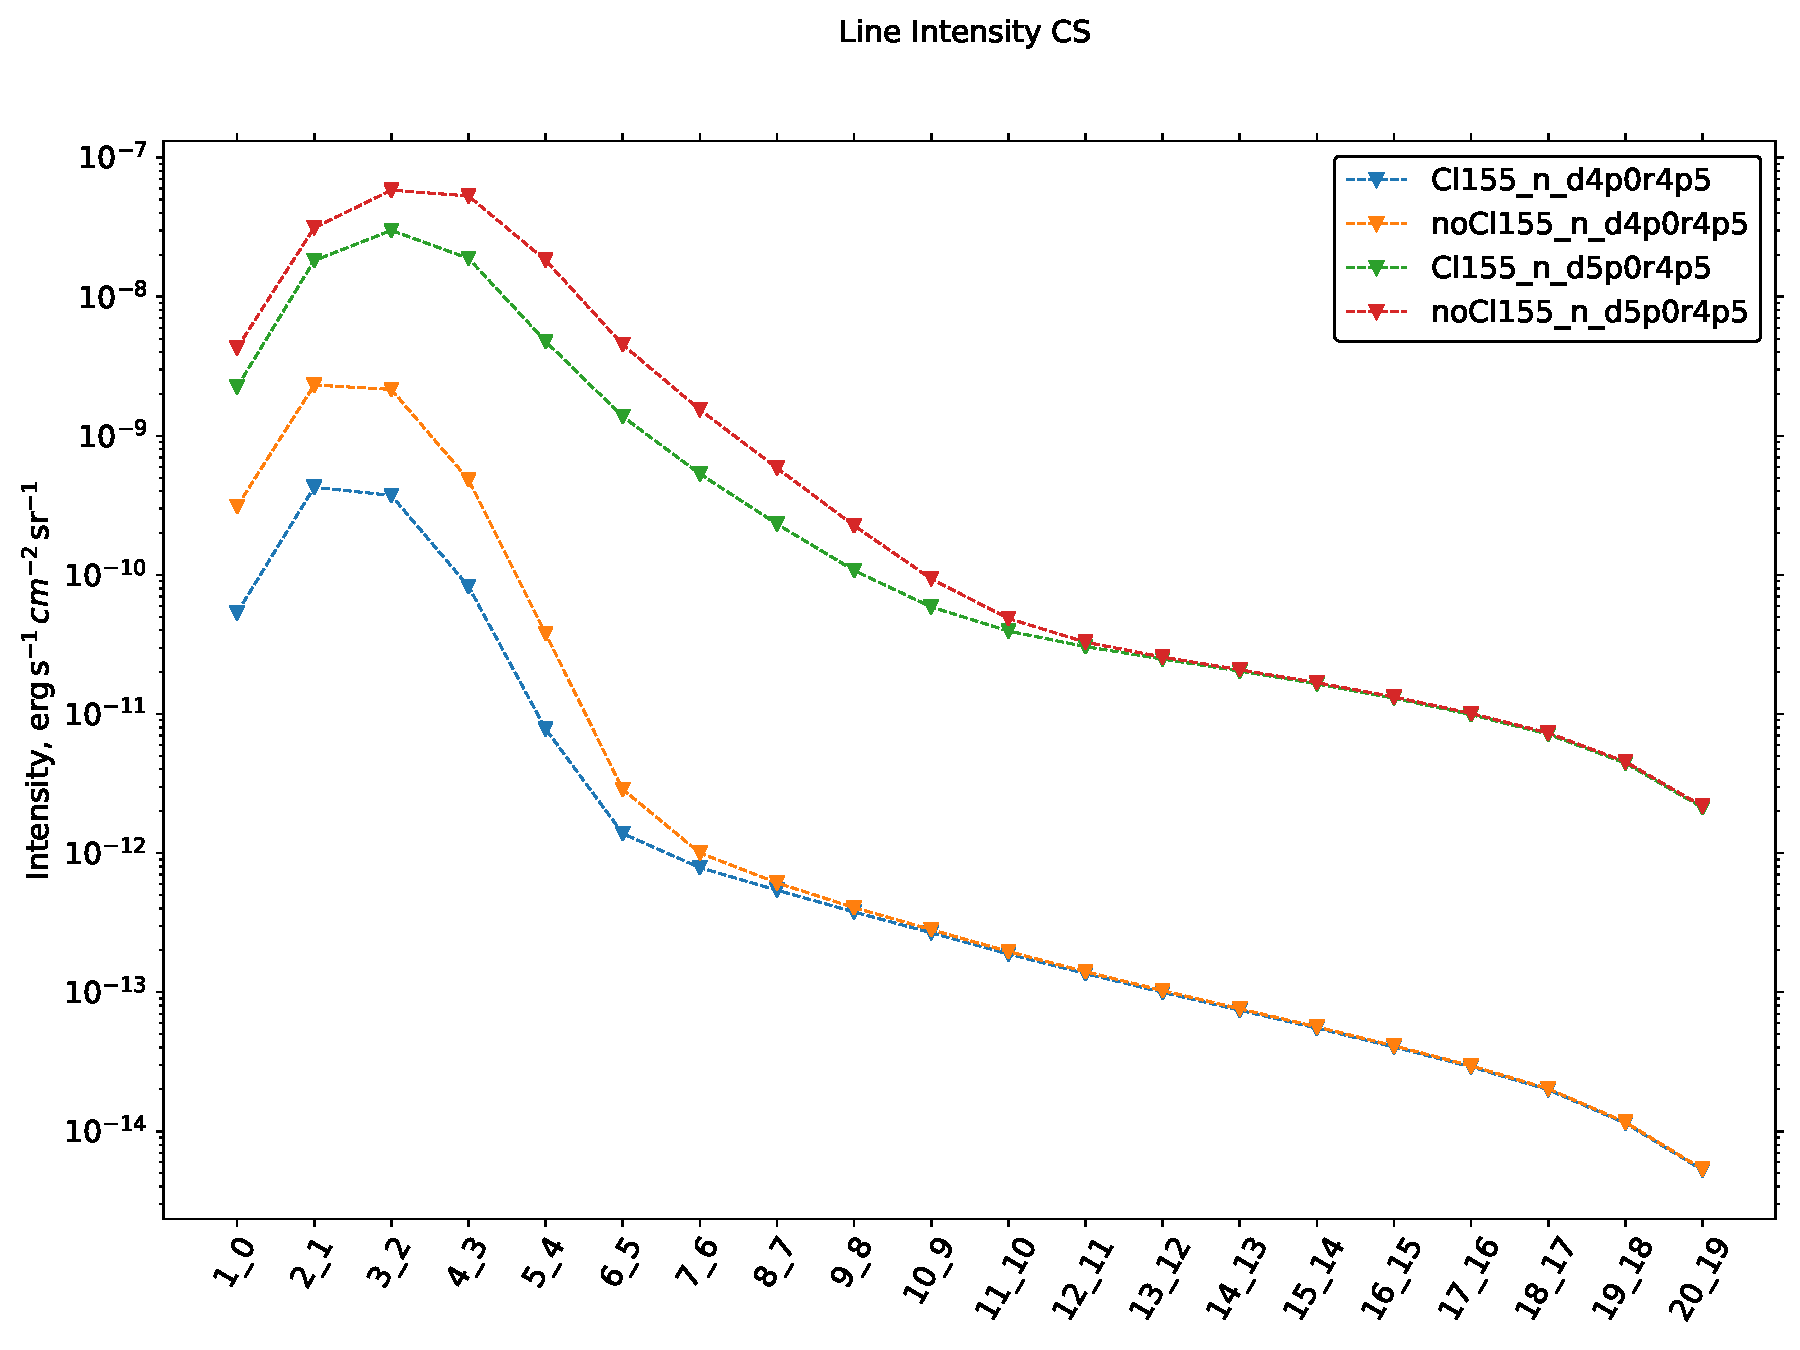
\includegraphics[trim = {0 0 0 1cm},clip,width=1\textwidth]{figure/Cl/gridModelEmiss/I_comp_CS.pdf}
        \caption{Diagramme d'intensité du $\mathrm{CS}$}
        \label{fig:cl:emiss:CS}
\end{figure}

\begin{figure}[!h]
        \centering 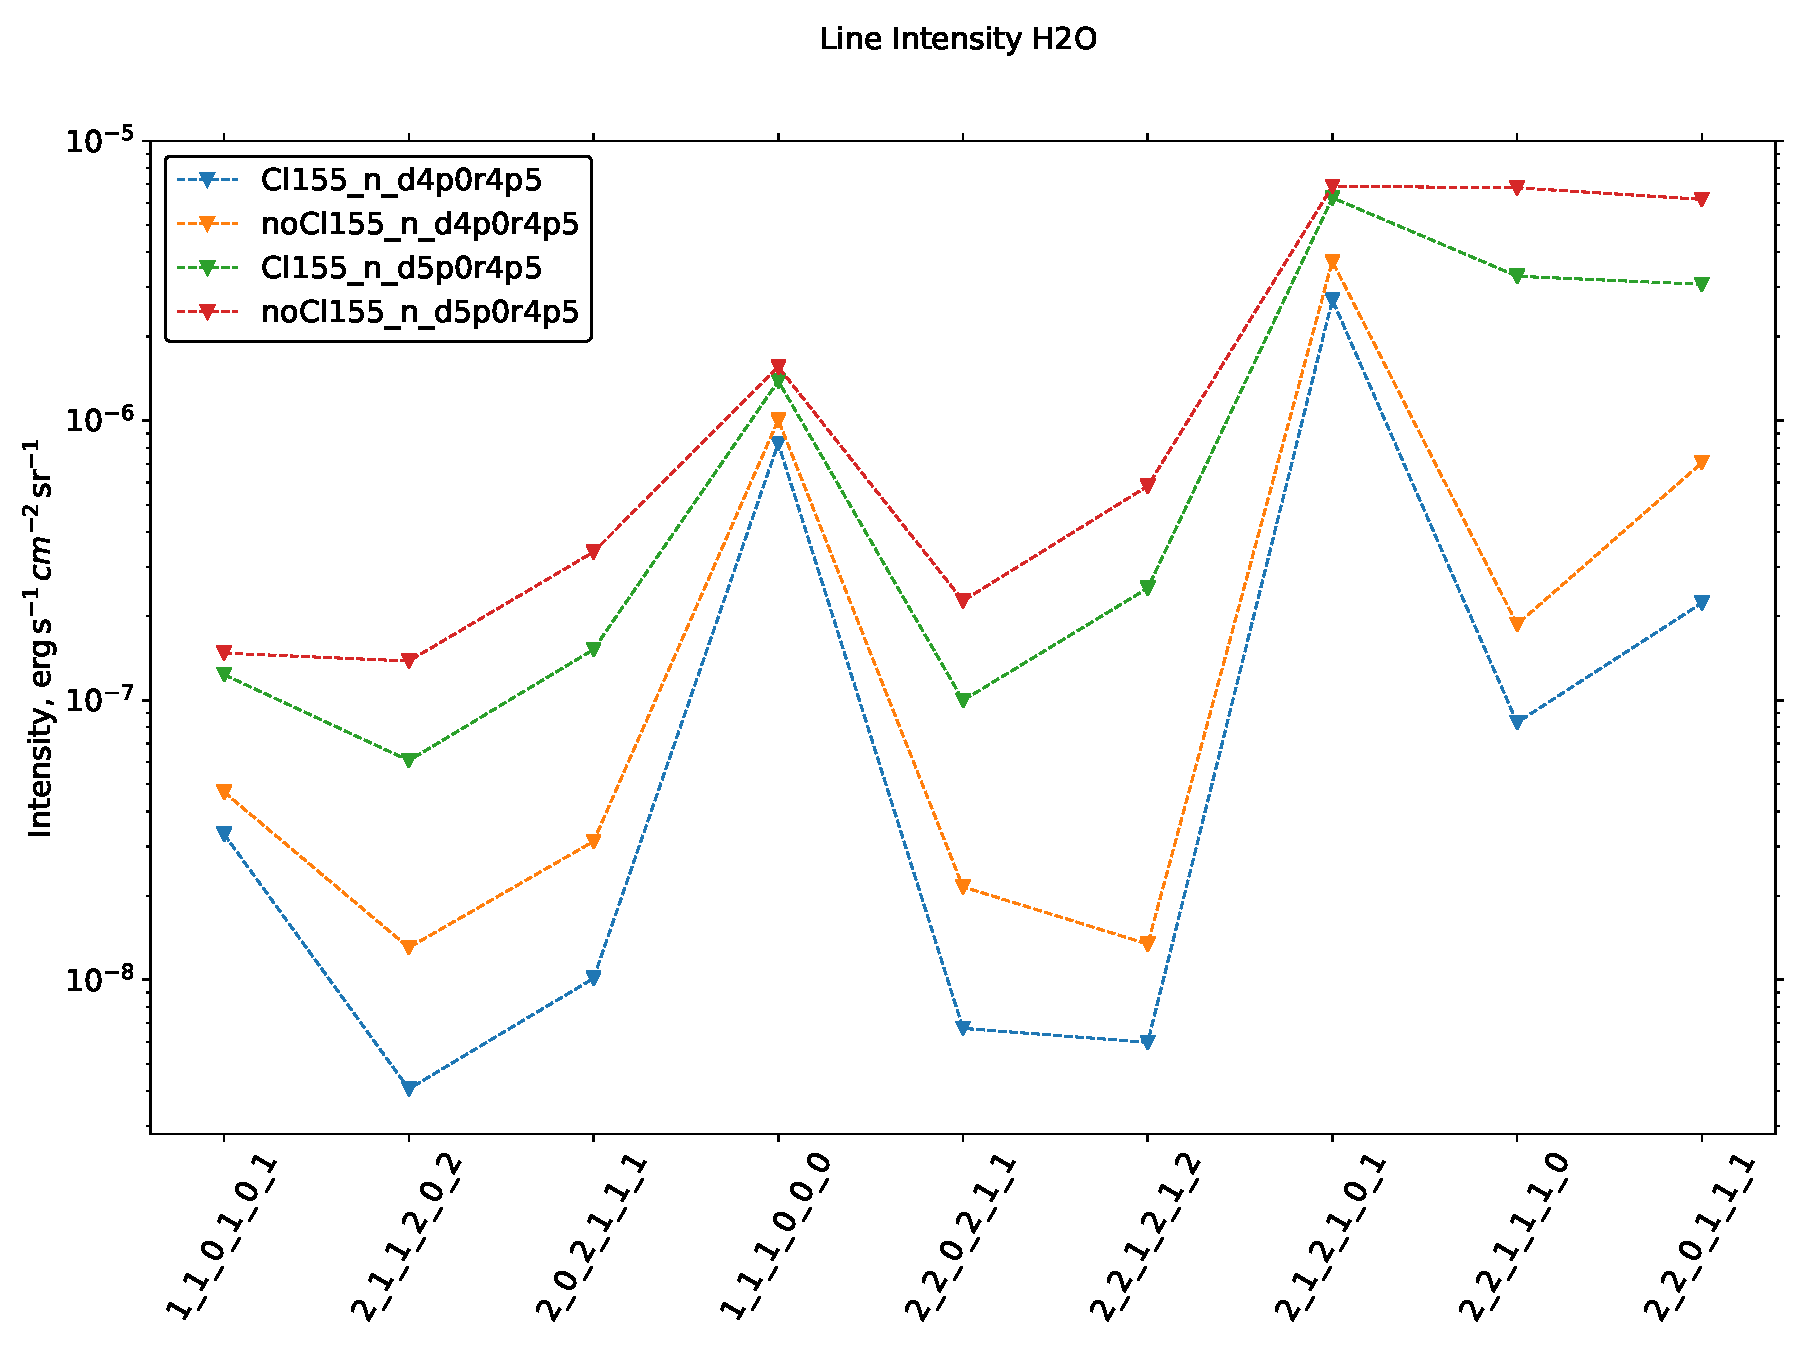
\includegraphics[trim = {0 0 0 1cm},clip,width=1\textwidth]{figure/Cl/gridModelEmiss/I_comp_H2O.pdf}
        \caption{Diagramme d'intensité du $\mathrm{H}_2\mathrm{O}$}
        \label{fig:cl:emiss:H2O}
\end{figure}

\begin{figure}[!h]
        \centering 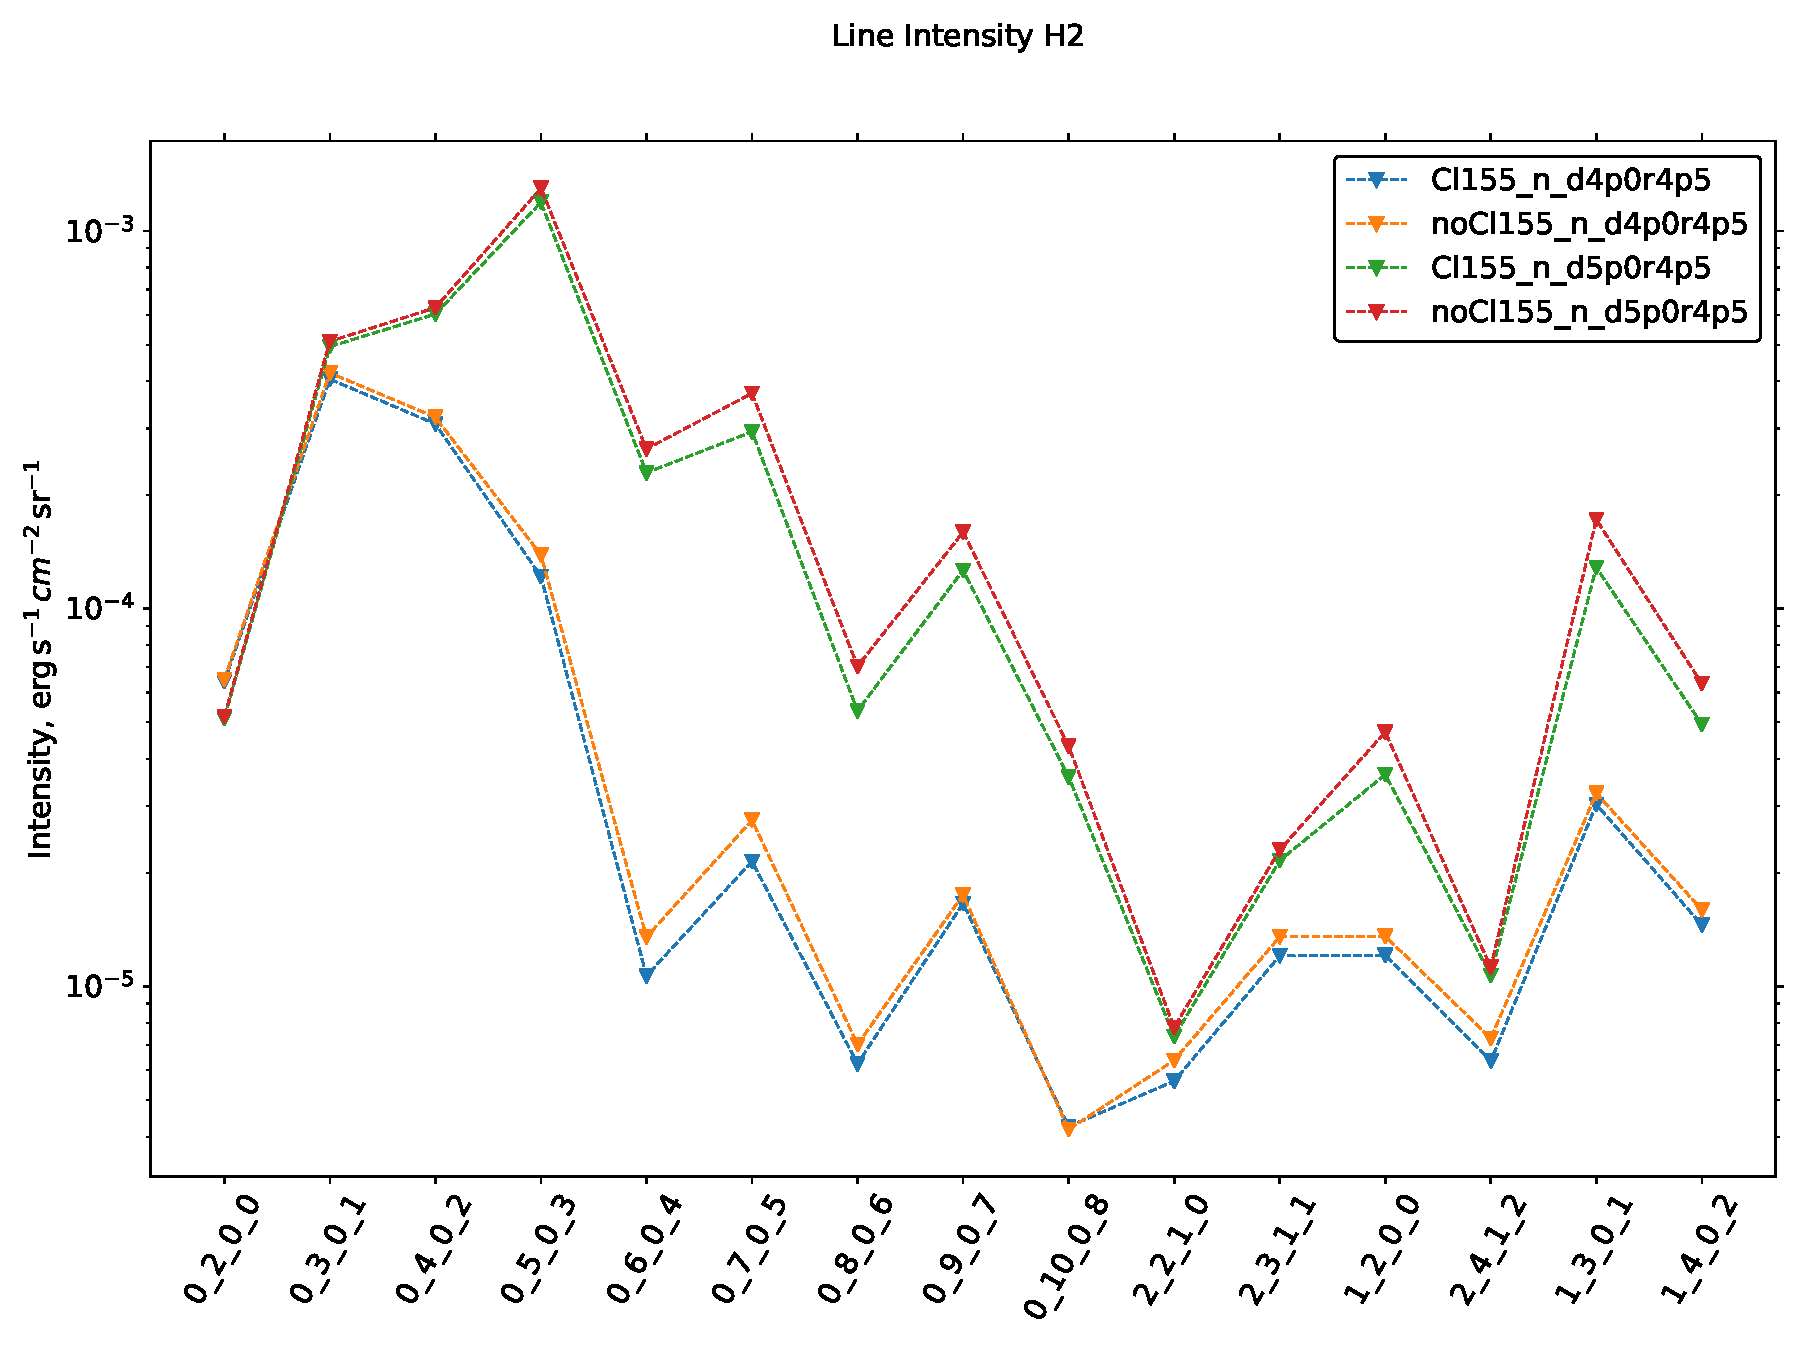
\includegraphics[trim = {0 0 0 1cm},clip,width=1\textwidth]{figure/Cl/gridModelEmiss/I_comp_H2.pdf}
        \caption{Diagramme d'intensité du $\mathrm{H}_2$}
        \label{fig:cl:emiss:H2}
\end{figure}

\begin{figure}[!h]
        \centering 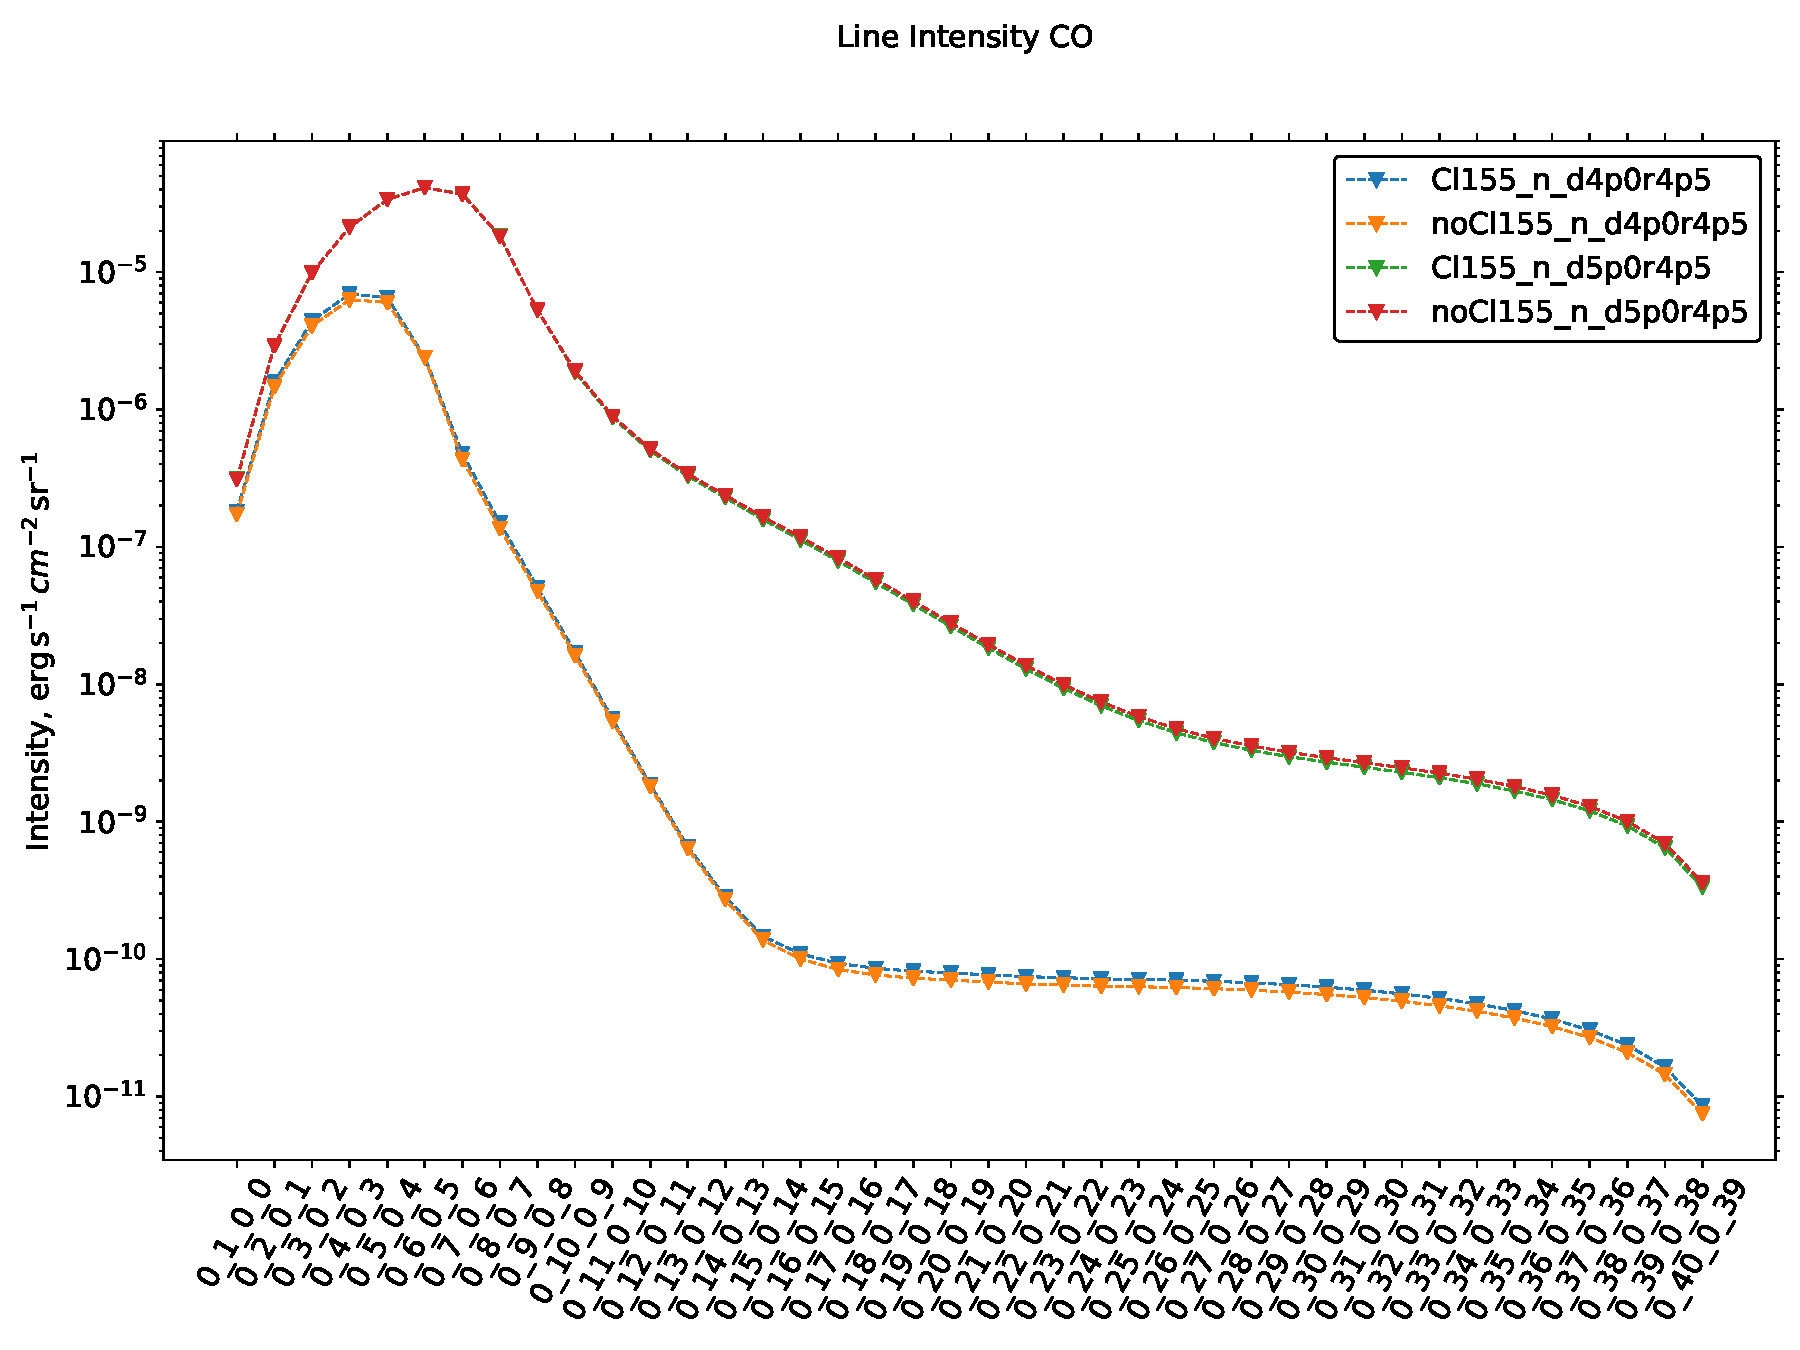
\includegraphics[trim = {0 0 0 1cm},clip,width=1\textwidth]{figure/Cl/gridModelEmiss/I_comp_CO.pdf}
        \caption{Diagramme d'intensité du $\mathrm{CO}$. Seules les transitions rotationnelles ont été écrites (toutes s'effectuent à $\mathrm{v}=0$)}
        \label{fig:cl:emiss:CO}
\end{figure}


\begin{figure}[!h]
    \centering
    \begin{subfigure}[t]{0.49\textwidth} % "0.49" donne ici la largeur de l'image
        \centering 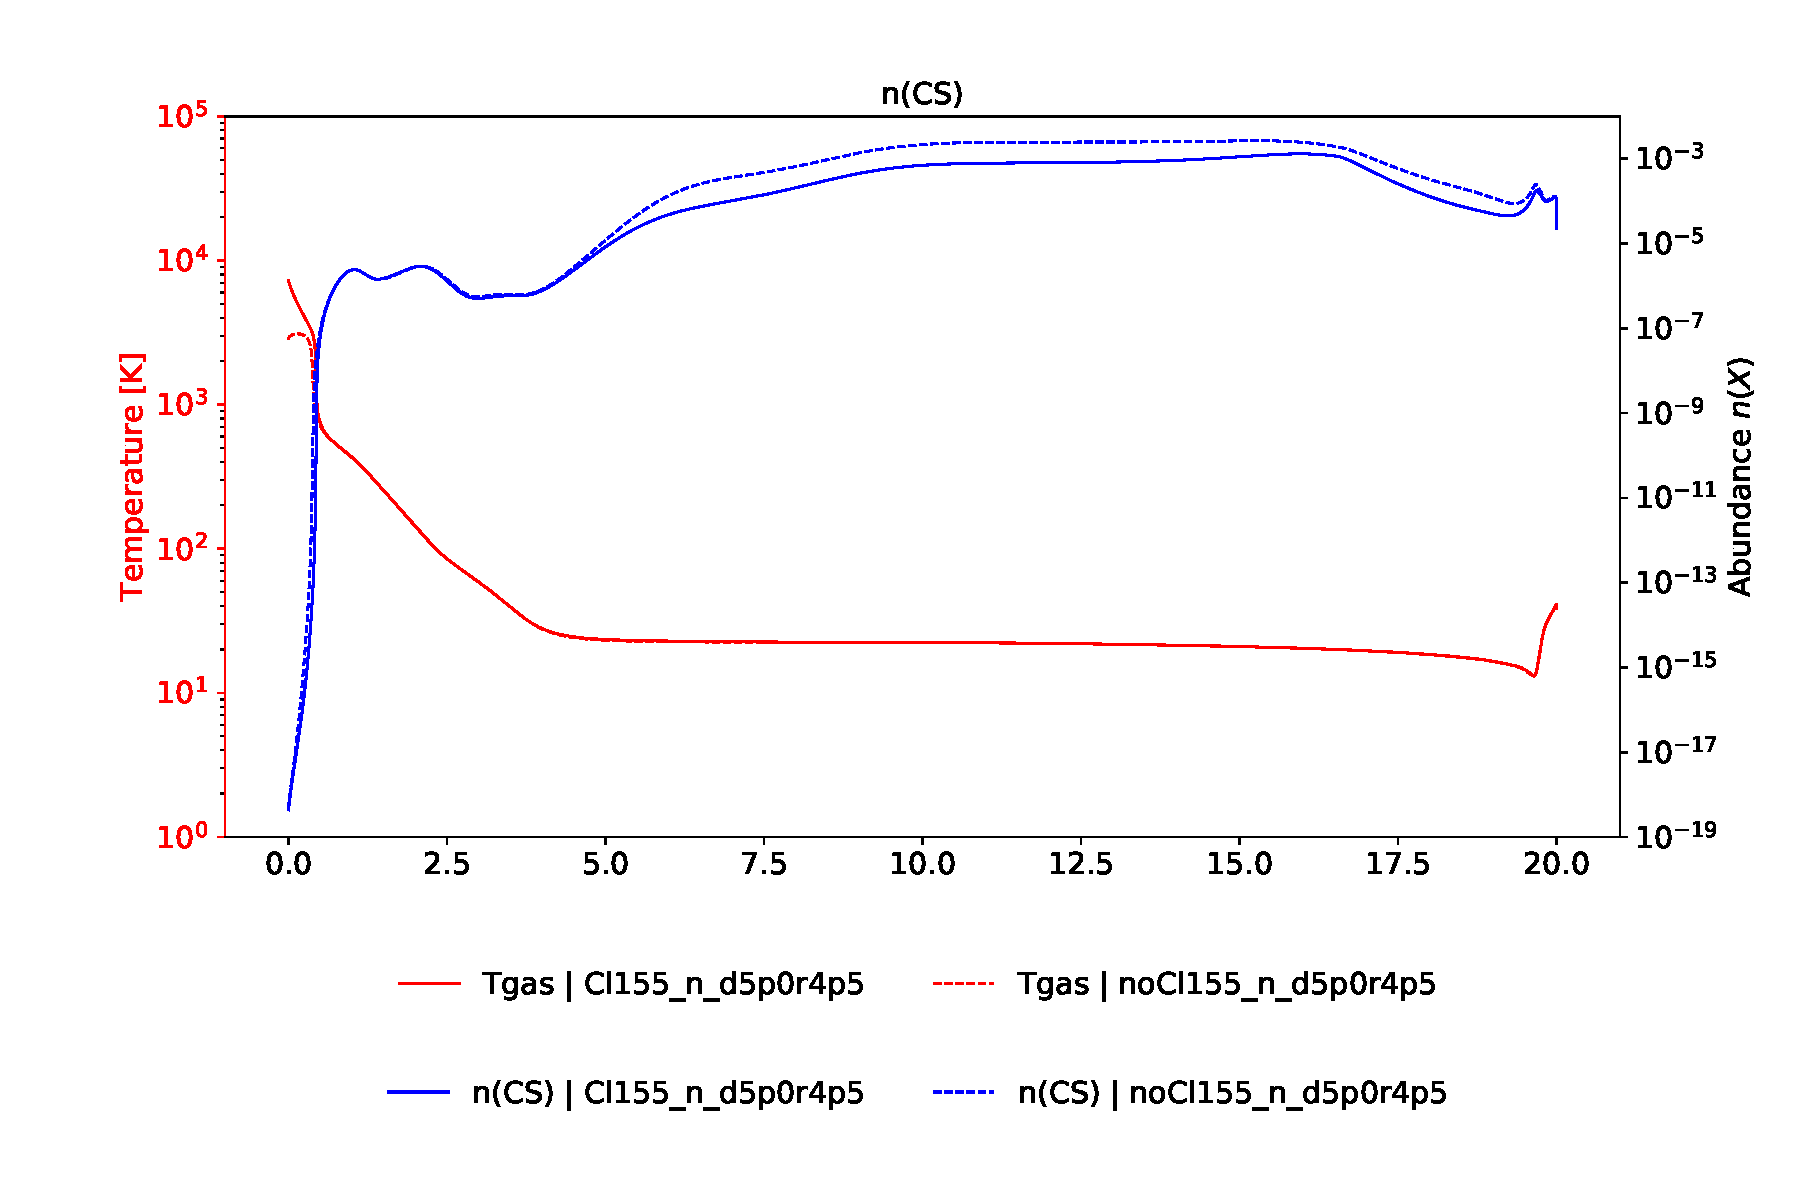
\includegraphics[trim = {0 0 0 0},clip,width=1\textwidth]{figure/Cl/gridModelEmiss/nT_comp_CS.pdf}
        \caption{$\mathrm{CS}$}
    \end{subfigure}
    ~ 
   \begin{subfigure}[t]{0.49\textwidth} % "0.49" donne ici la largeur de l'image
        \centering 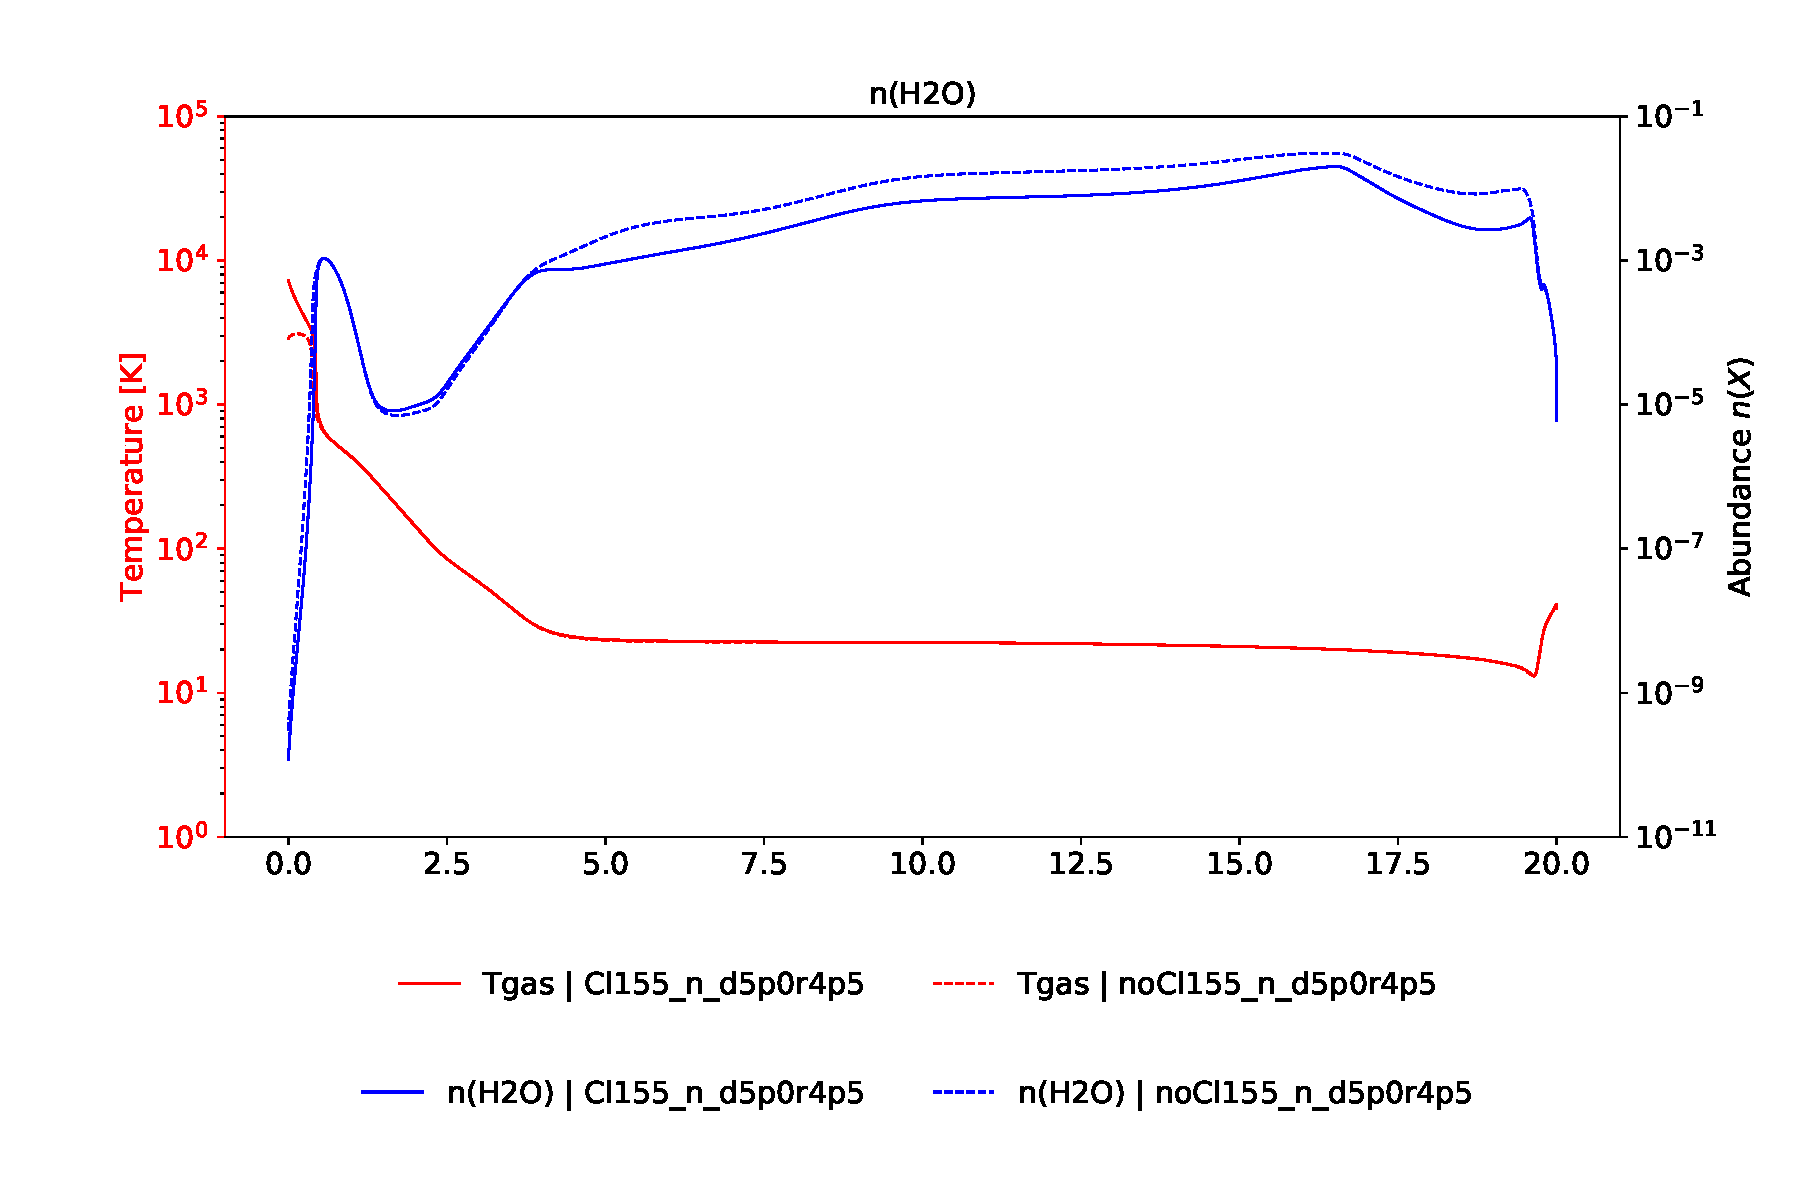
\includegraphics[trim = {0 0 0 0},clip,width=1\textwidth]{figure/Cl/gridModelEmiss/nT_comp_H2O.pdf}
        \caption{$\mathrm{H}_2\mathrm{O}$}
    \end{subfigure}
    
    \begin{subfigure}[t]{0.49\textwidth} % "0.49" donne ici la largeur de l'image
        \centering 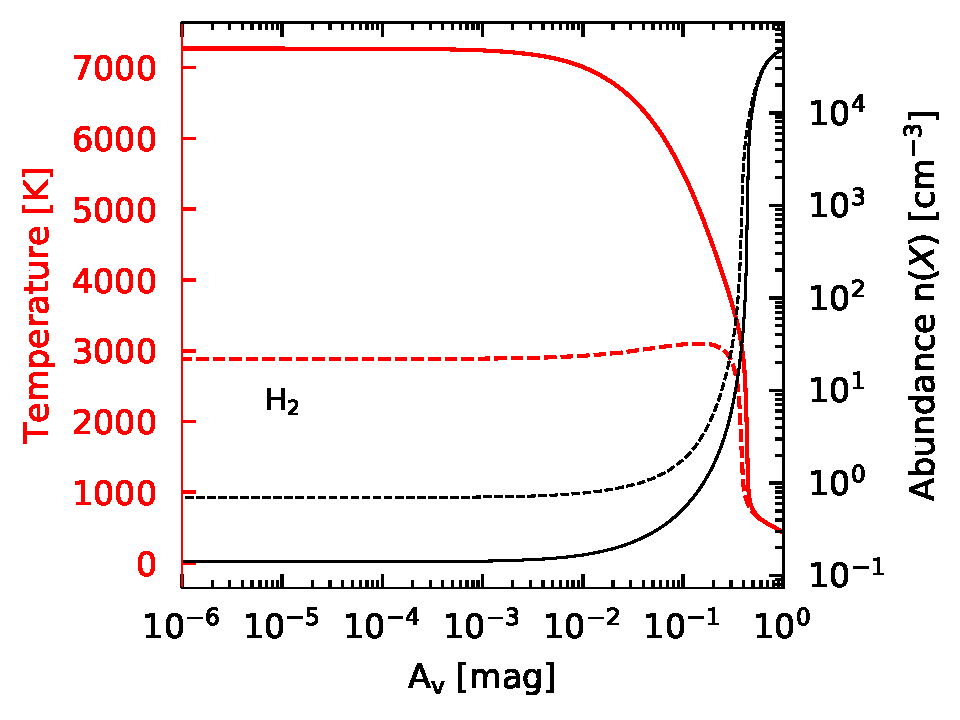
\includegraphics[trim = {0 0 0 0},clip,width=1\textwidth]{figure/Cl/gridModelEmiss/nT_comp_H2.pdf}
        \caption{$\mathrm{H}_2$}
    \end{subfigure}
    ~ 
    \begin{subfigure}[t]{0.49\textwidth} % "0.49" donne ici la largeur de l'image
        \centering 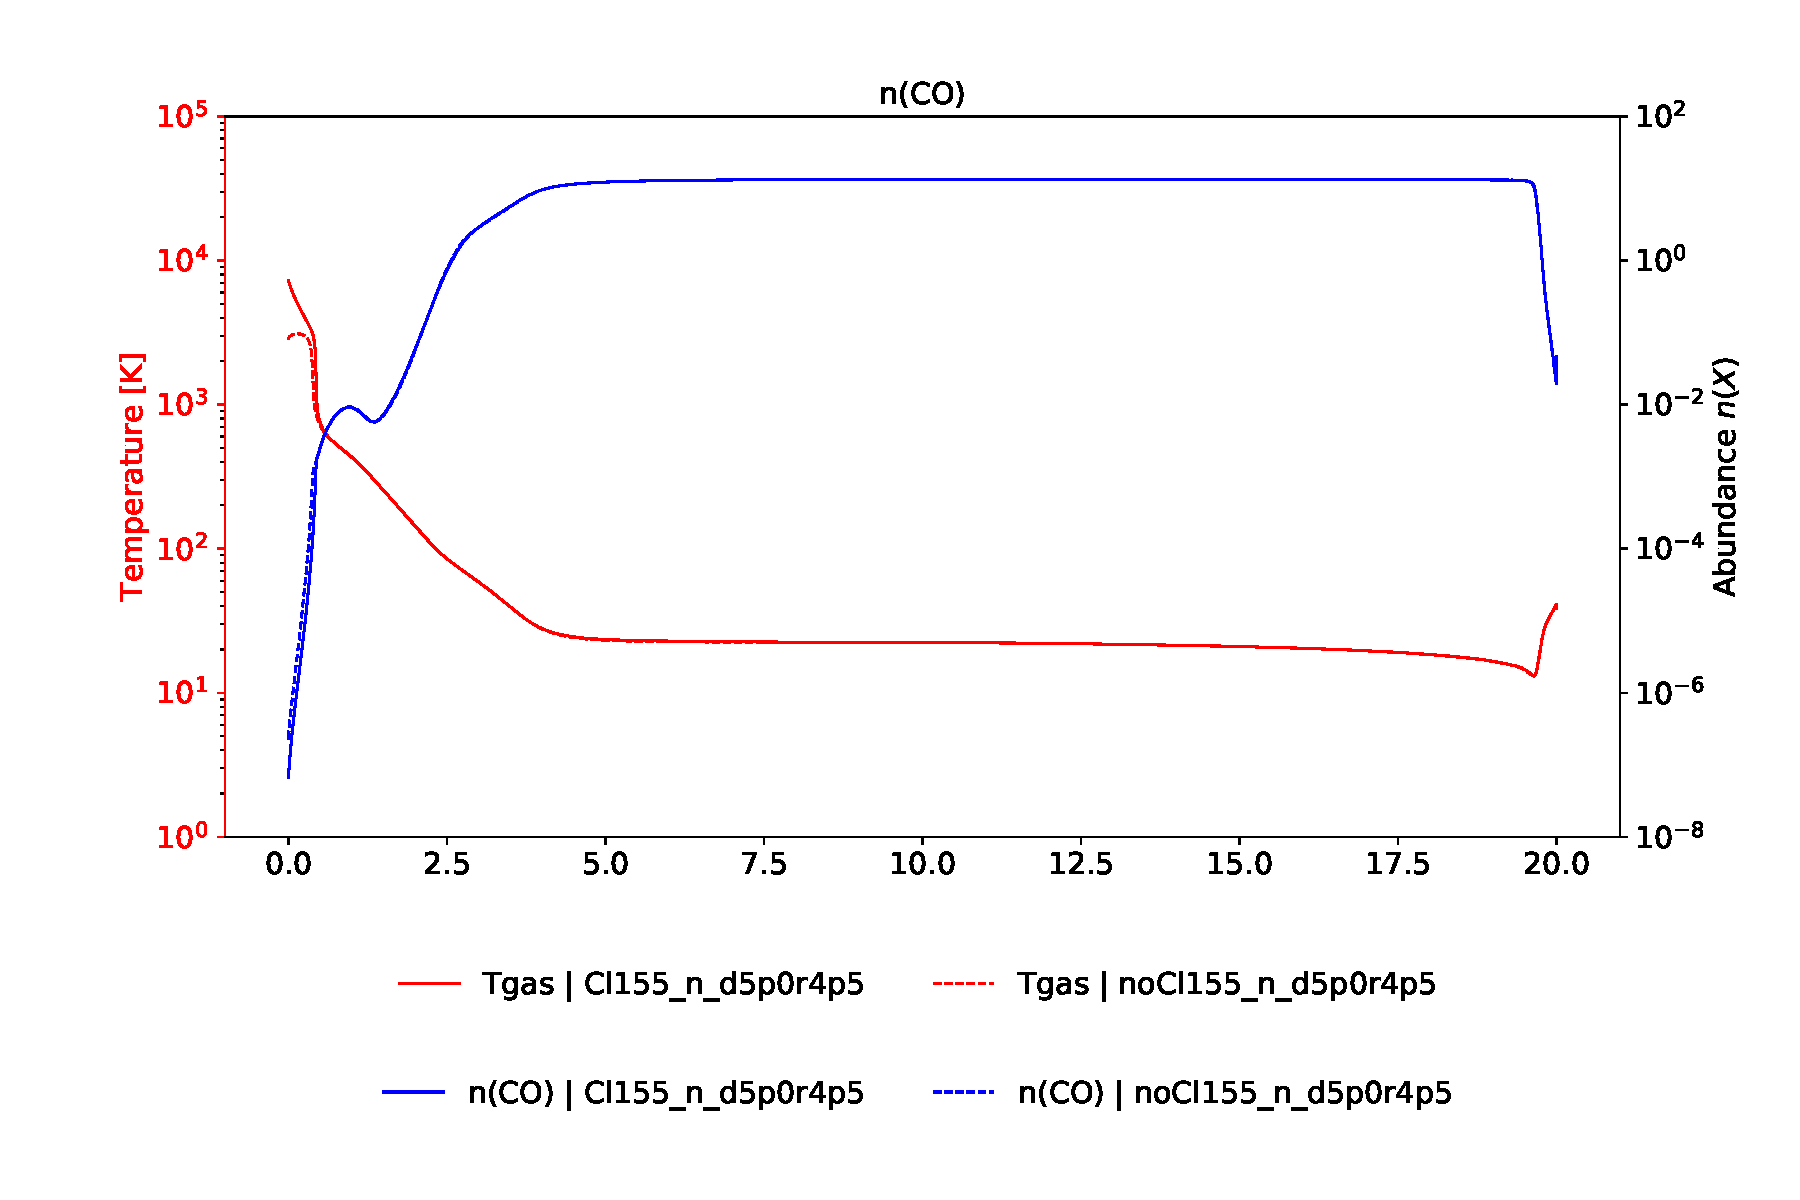
\includegraphics[trim = {0 0 0 0},clip,width=1\textwidth]{figure/Cl/gridModelEmiss/nT_comp_CO.pdf}
        \caption{$\mathrm{CO}$}
    \end{subfigure}
    
    \caption{Profils de densité et de températures des traceurs impactés par l'ajout du chlore. Mêmes conventions que pour la figure \ref{fig:Cl:gridModelEmiss:nT:yes}. Les traceurs moléculaires sont peu modifiés par l'augmentation de la température de la zone atomique du nuage. }
    \label{fig:Cl:gridModelEmiss:nT:no}
\end{figure}


%%%%%%%%%%%%%%%%%%%%%%%%%%%%%%%%%%%%%%%%%%%%%%%%%%%%%%%%%%%%%%%%%%%%%%%%%%%%%%%%%%%%%%%%%%%%%
\clearpage
\section{Réactions chimiques initiées par $\mathrm{H}_2$}
\label{appendix:type46}
\begin{figure}[!h]
    \centering 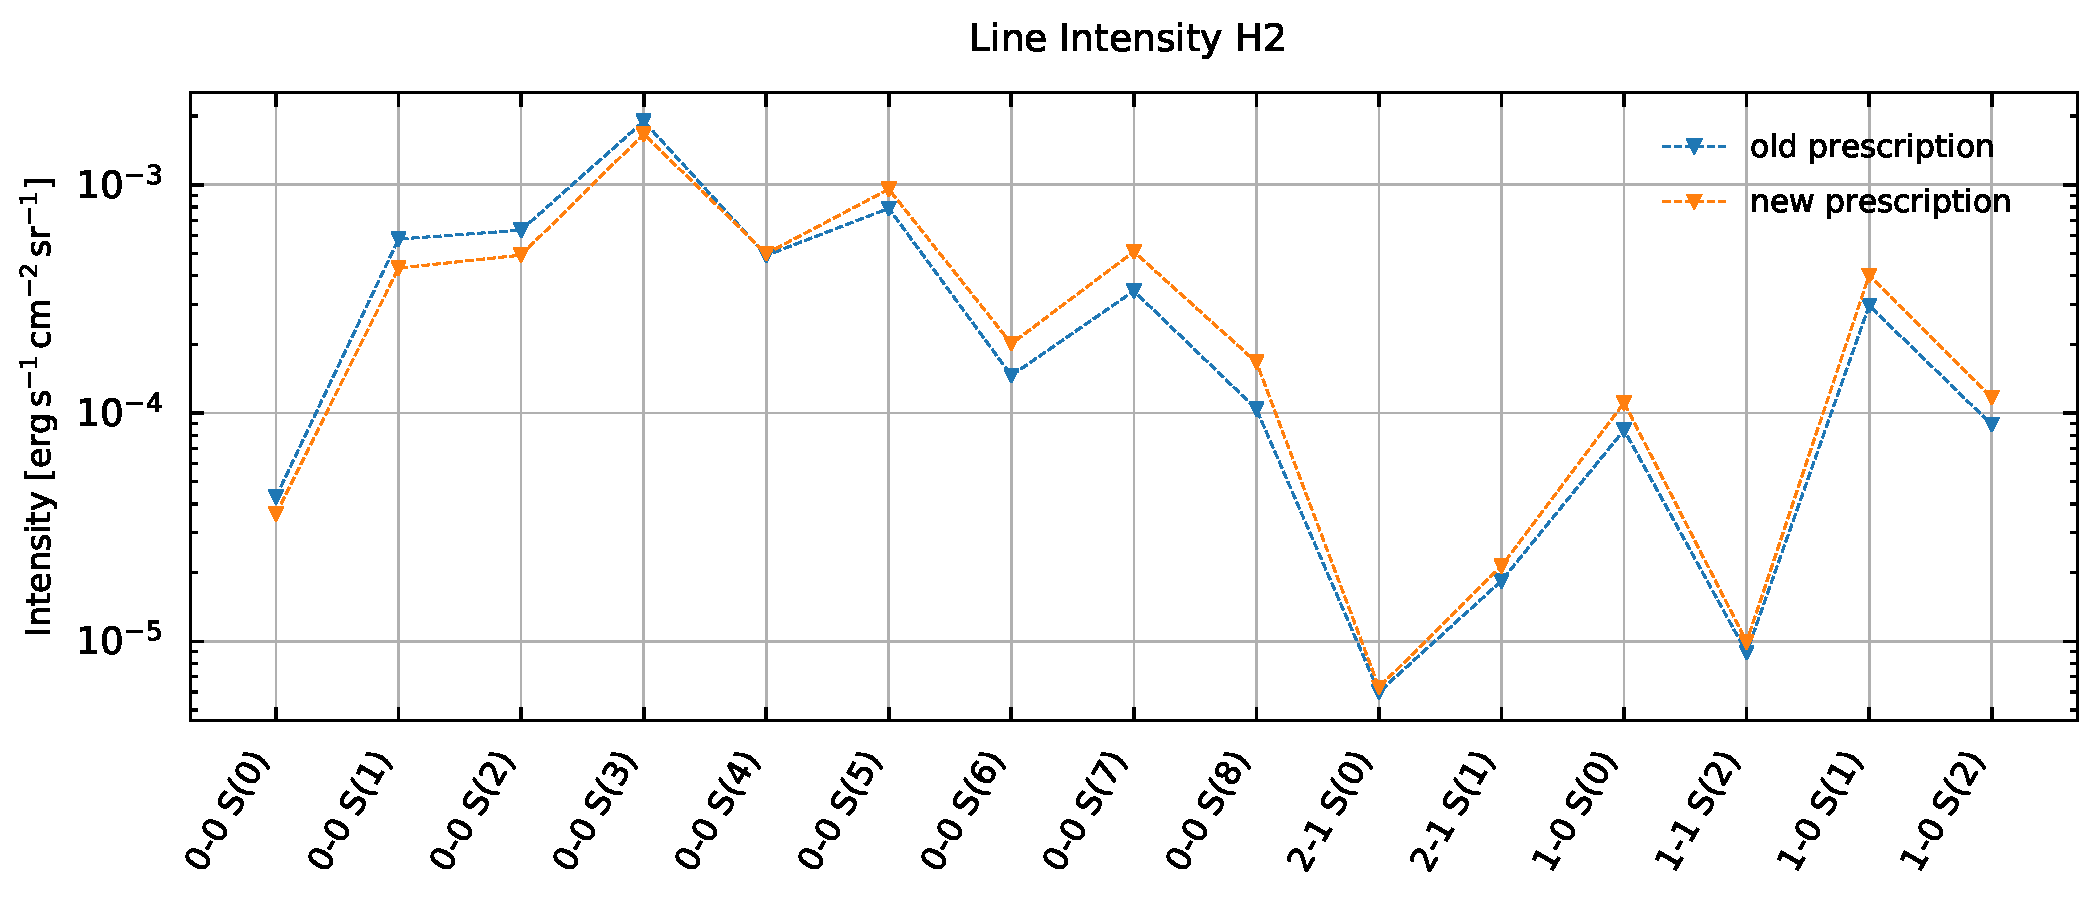
\includegraphics[trim = {0 0 0 1cm},clip,width=1\textwidth]{figure/type46/I_comp_H2.pdf}
    \caption{Diagramme d'intensité du $\mathrm{H}_2$}
    \begin{minipage}{\textwidth}
    
    \end{minipage}
    \label{fig:type46:H2}
\end{figure}

\begin{figure}[!h]
    \centering 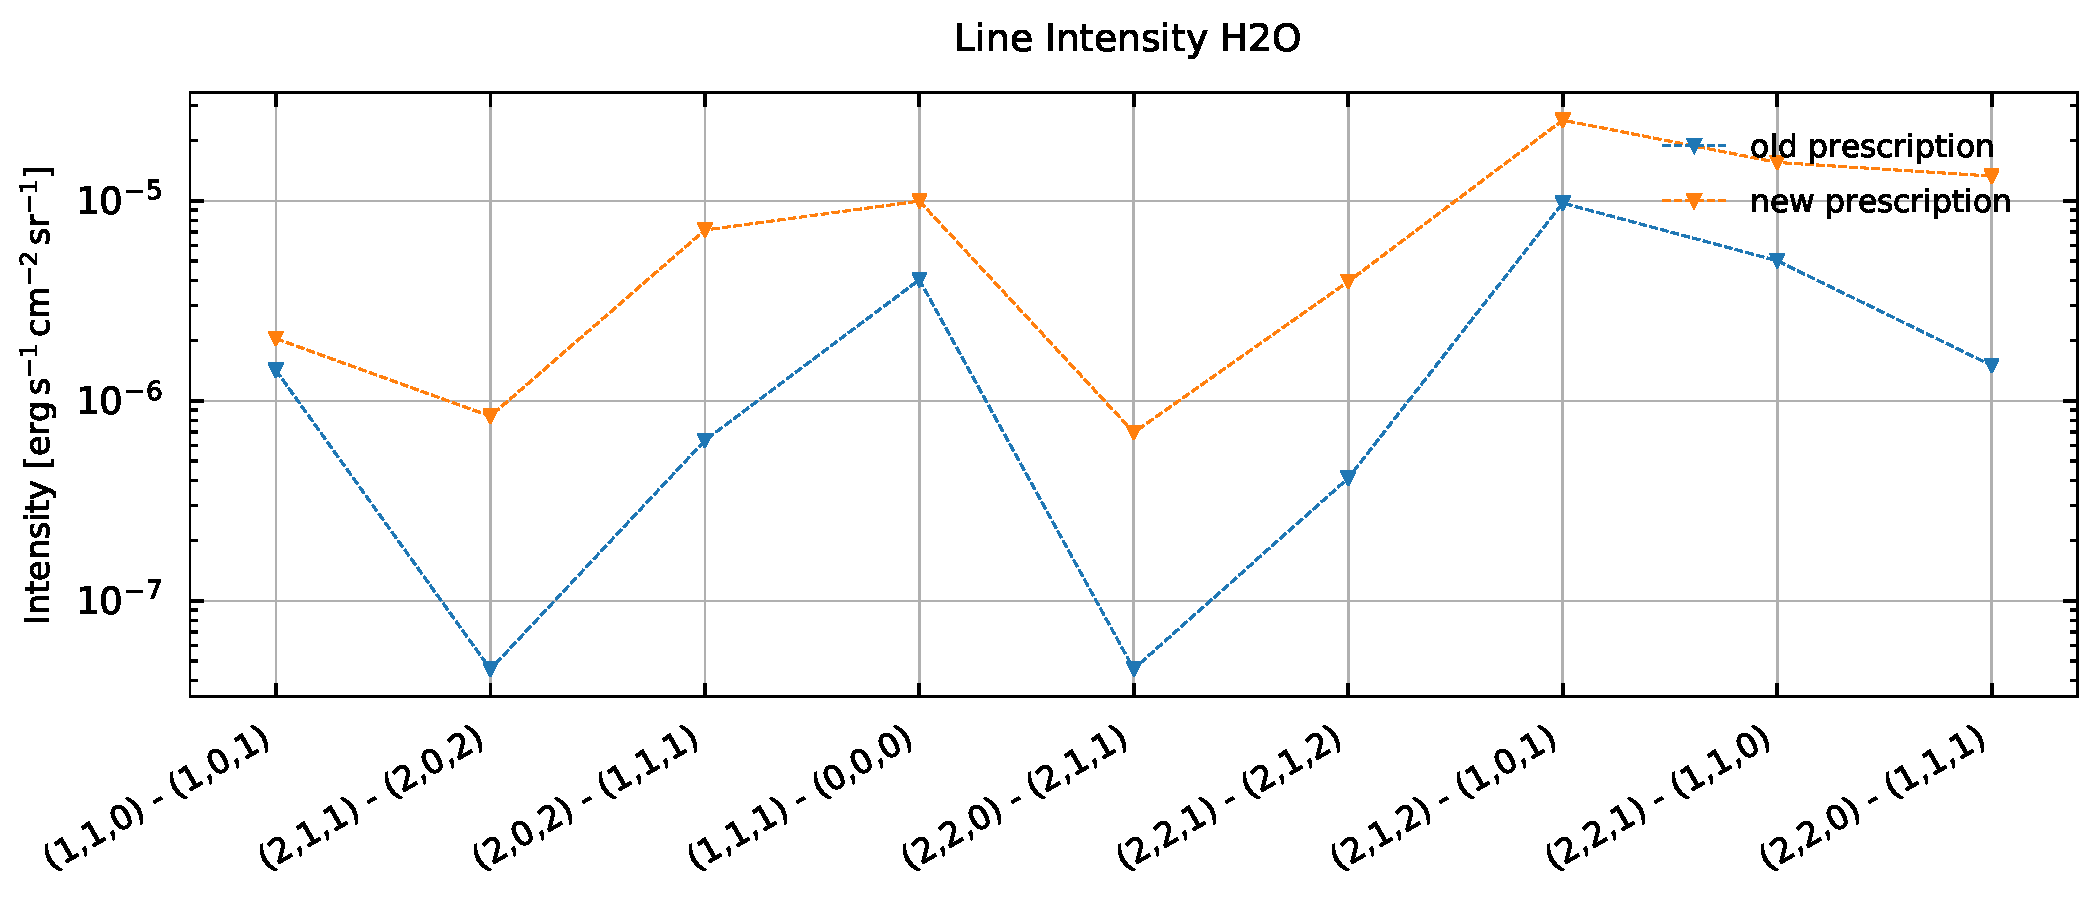
\includegraphics[trim = {0 0 0 1cm},clip,width=1\textwidth]{figure/type46/I_comp_H2O.pdf}
    \caption{Diagramme d'intensité du $\mathrm{H}_2\mathrm{O}$}
    \begin{minipage}{\textwidth}
  
    \end{minipage}
    \label{fig:type46:H2O}
\end{figure}

\begin{figure}[!h]
    \centering 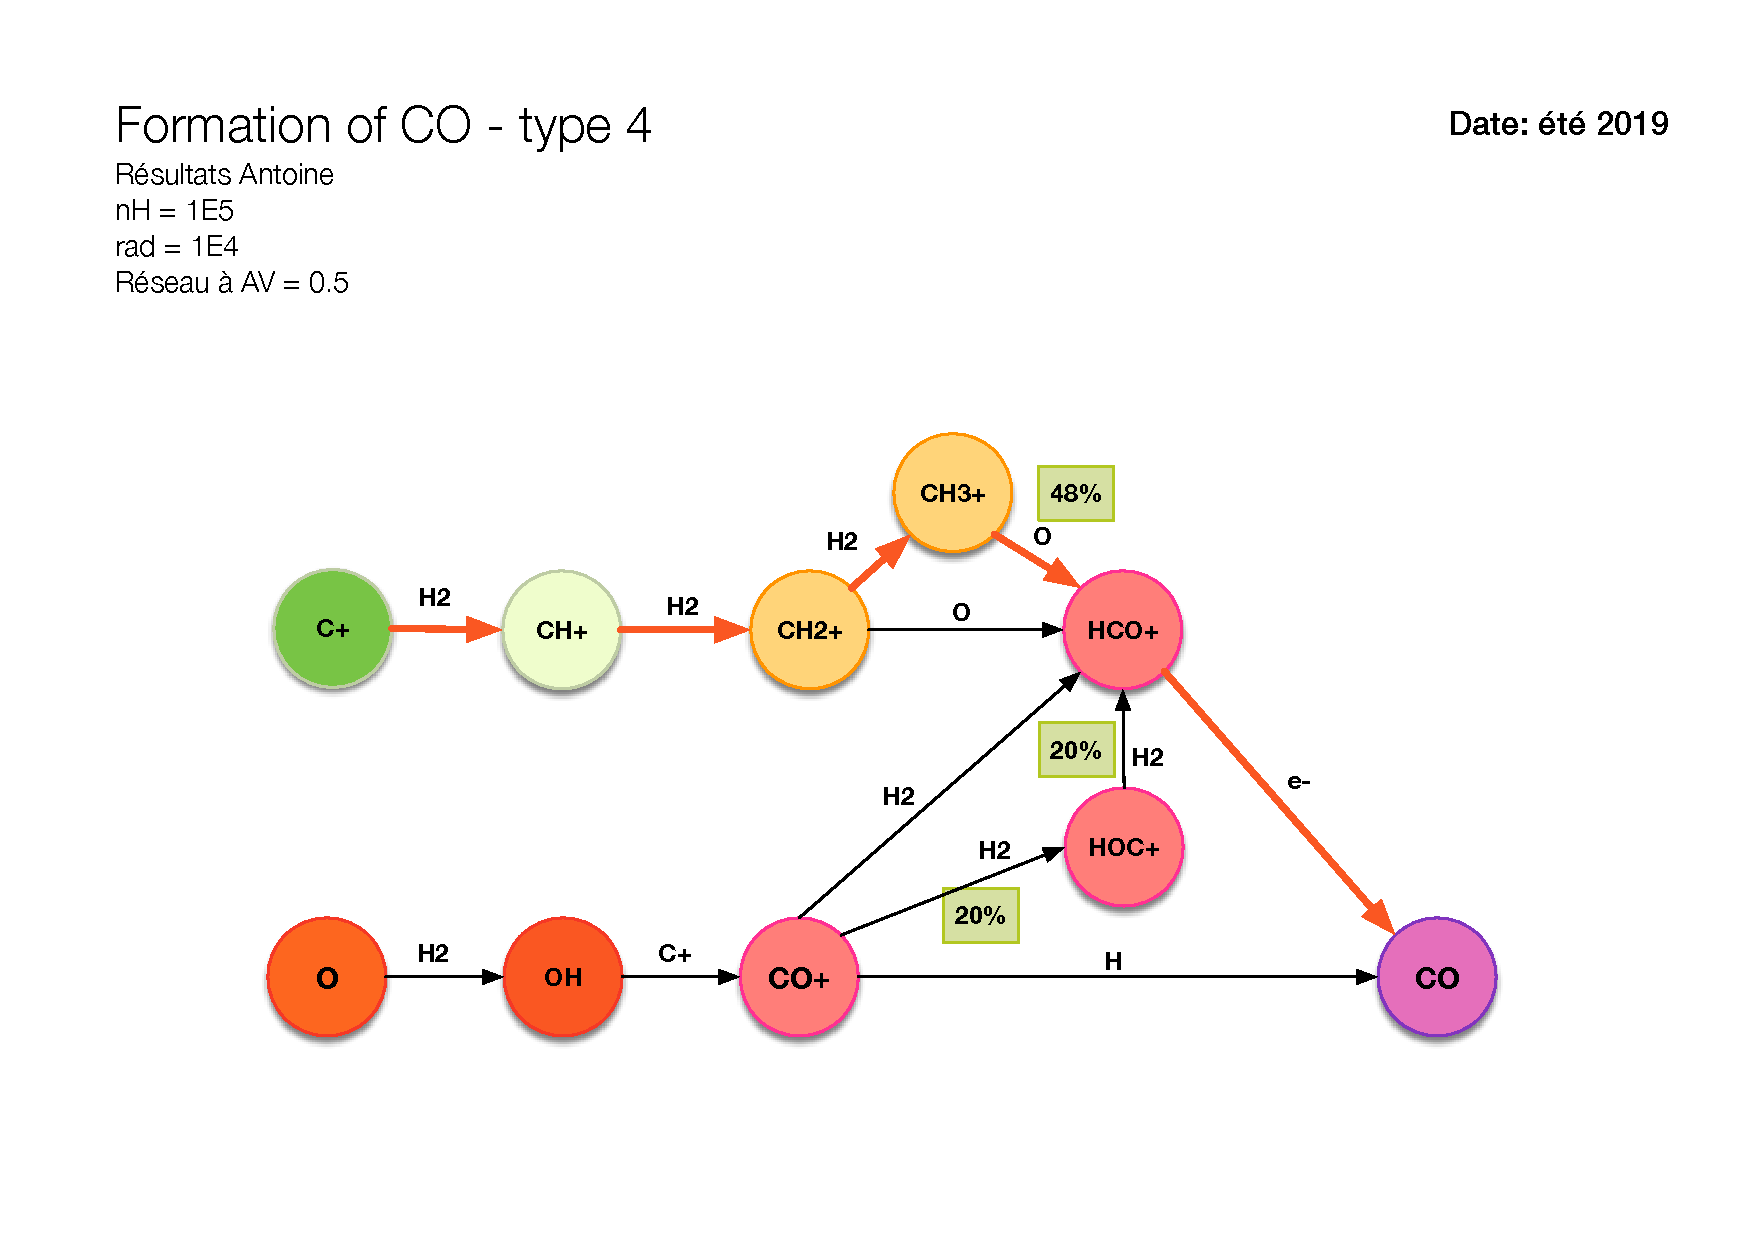
\includegraphics[trim = {3cm 3cm 3cm 7cm},clip,width=0.8\textwidth]{figure/type46/ChimieCO_1.pdf}
    \caption{Ancien réseau de formation du $\mathrm{CO}$}
    \label{fig:type46:form:COold}
\end{figure}


%%%%%%%%%%%%%%%%%%%%%%%%%%%%%%%%%%%%%%%%%%%%%%%%%%%%%%%%%%%%%%%%%%%%%%%%%
\clearpage
\section{Impact de la prescription de Glover}

% On a rassemblé dans cette section les figures servant à l'analyse mais qui sont trop volumineuse dans le rapport.

\vfill
\begin{figure}[!h]
    \centering
    \begin{subfigure}[t]{0.49\textwidth} % "0.49" donne ici la largeur de l'image
        \centering 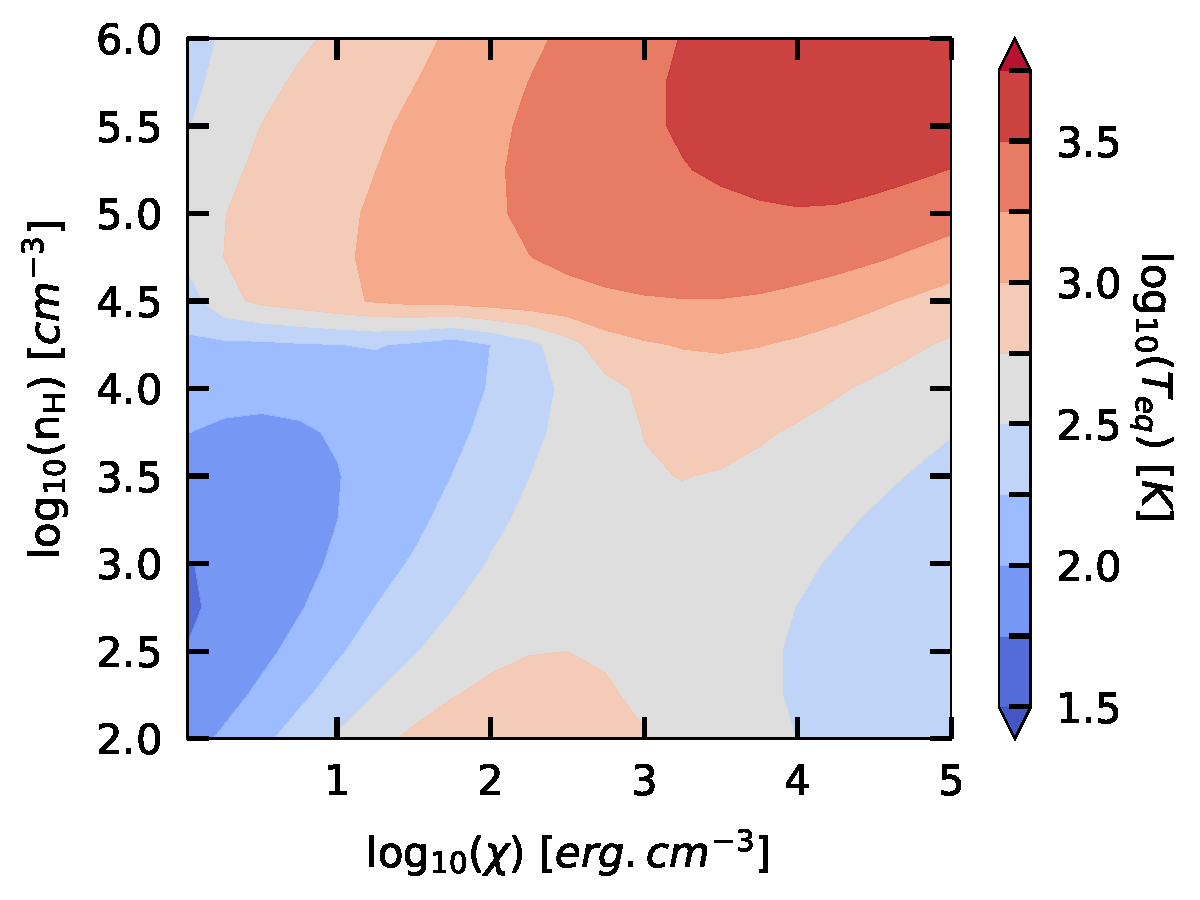
\includegraphics[trim = {0 0 0 0 },clip,width=1\textwidth]{figure/H2/grid_janev/mapTba.pdf}
        \caption{Prescription de Janev}
    \end{subfigure}
    ~ 
    \begin{subfigure}[t]{0.49\textwidth}
        \centering 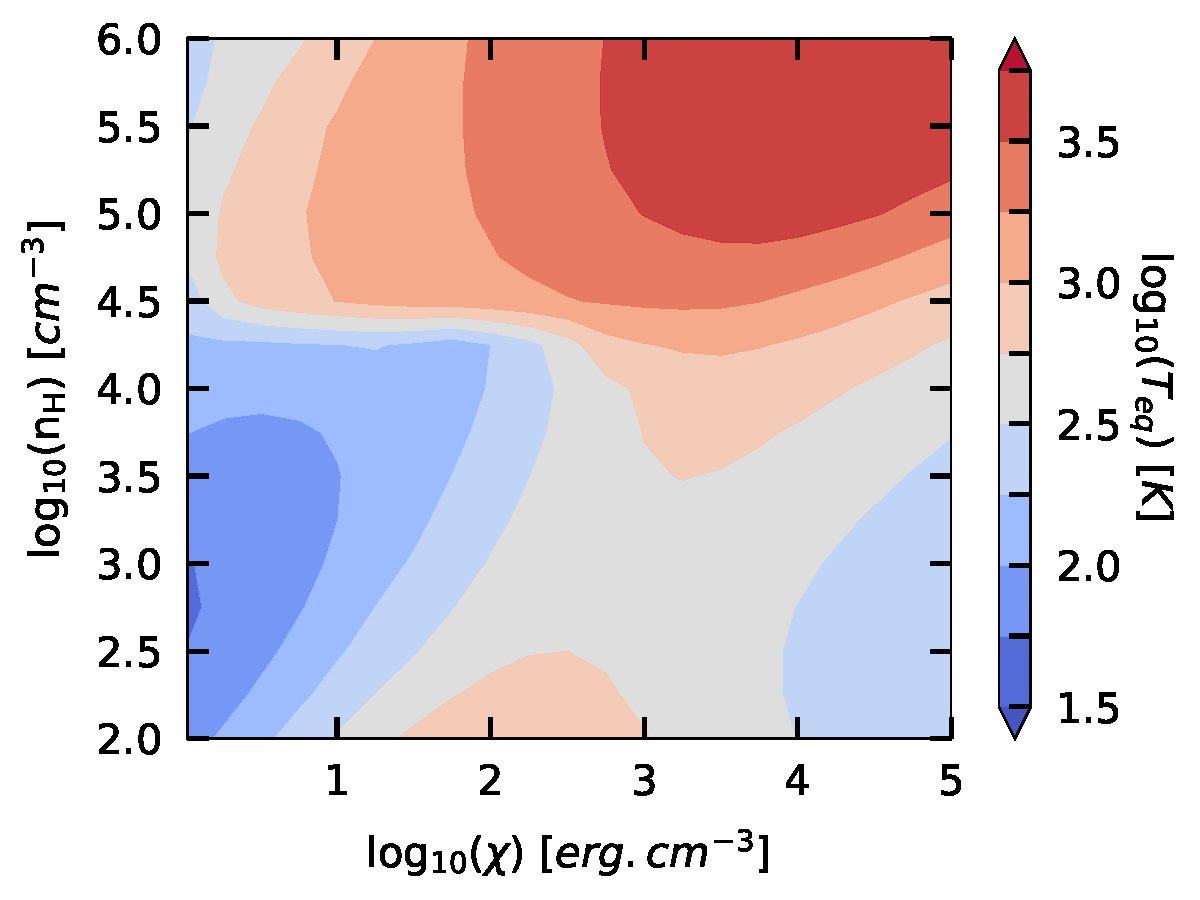
\includegraphics[trim = {0 0 0 0 },clip,width=1\textwidth]{figure/H2/grid_glover/mapTba.pdf}
        \caption{Prescription de Glover}
    \end{subfigure}
    \caption{Comparaison de la température en bord atomique de nuage pour des modèles utilisant la prescription de Janev et de Glover}
    \label{fig:H2:JanevGlover:Tba}
\end{figure}
\vfill

\begin{figure}[!p]
    \centering
    \begin{subfigure}[t]{0.49\textwidth} % "0.49" donne ici la largeur de l'image
        \centering 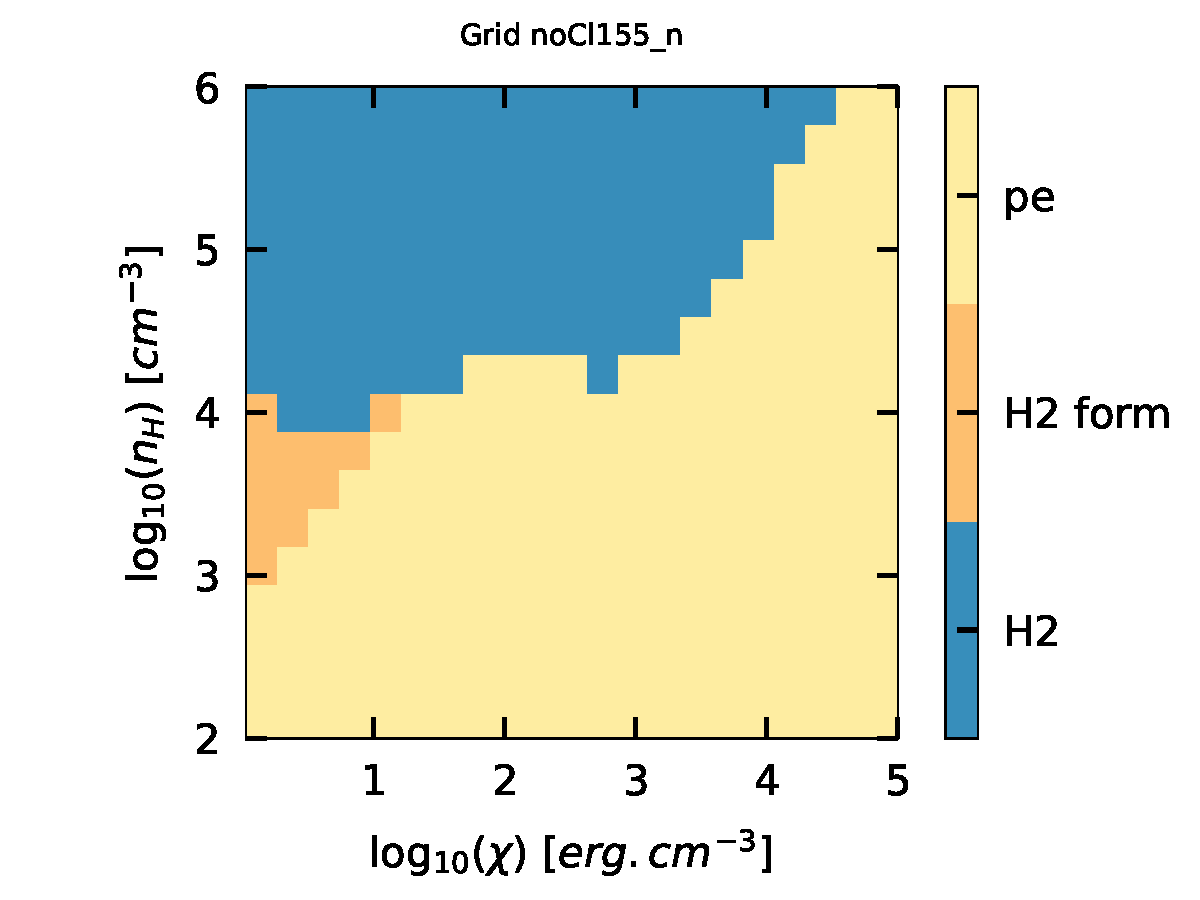
\includegraphics[trim = {0 0 0 1cm },clip,width=1\textwidth]{figure/H2/grid_janev/mapGmax.pdf}
        \caption{Prescription de Janev}
    \end{subfigure}
    ~ 
    \begin{subfigure}[t]{0.49\textwidth}
        \centering 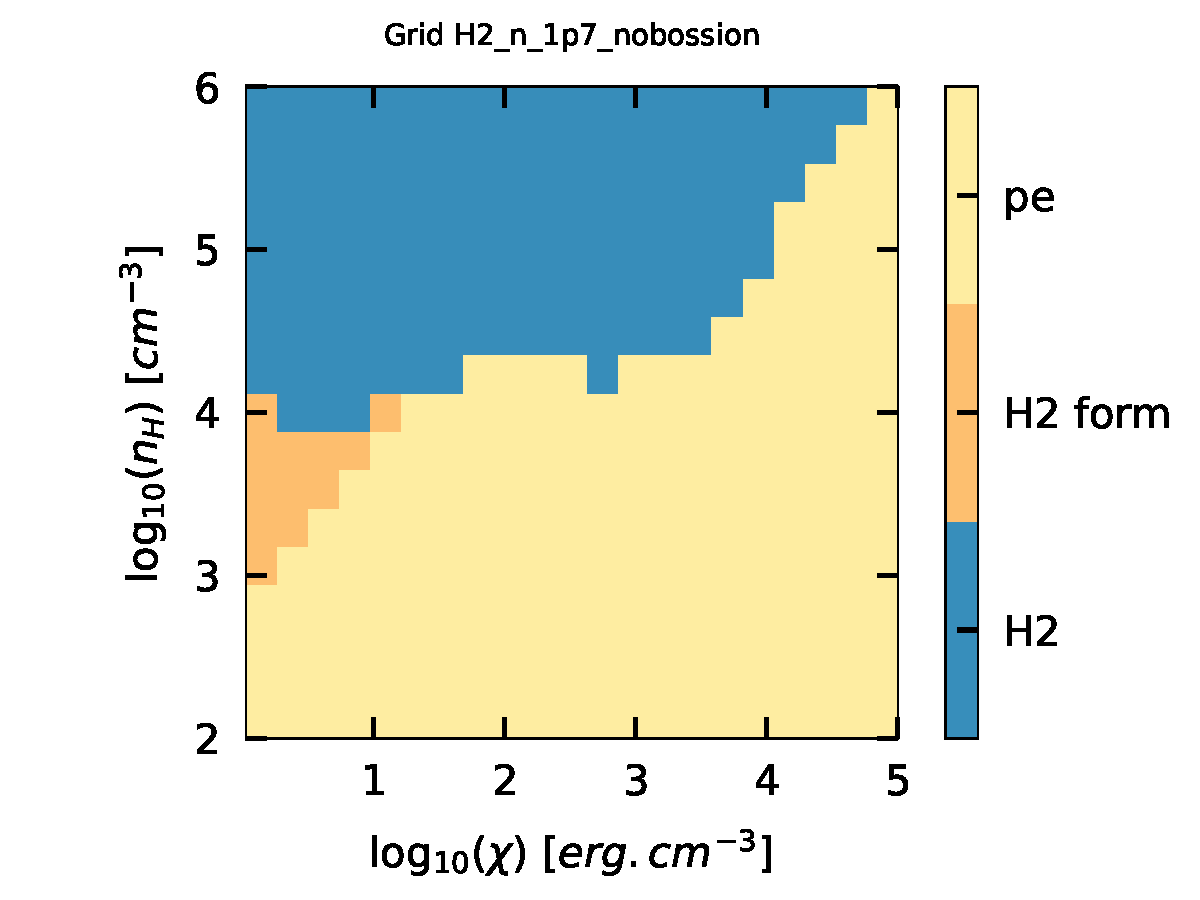
\includegraphics[trim = {0 0 0 1cm },clip,width=1\textwidth]{figure/H2/grid_glover/mapGmax.pdf}
        \caption{Prescription de Glover}
    \end{subfigure}
    \caption{Processus de chauffage dominant en bord de région atomique}
    \begin{minipage}{\textwidth}
    "pe" désigne le chauffage par effet photoélectrique sur les grains. "H2" désigne le chauffage par pompage UV de la molécule $\mathrm{H}_2$ et "H2 form" la formation de la molécule sur les grains.
    \end{minipage}
    \label{fig:H2:JanevGlover:Gmax}
    \hspace{1em}
    
    \begin{subfigure}[t]{0.49\textwidth} % "0.49" donne ici la largeur de l'image
        \centering 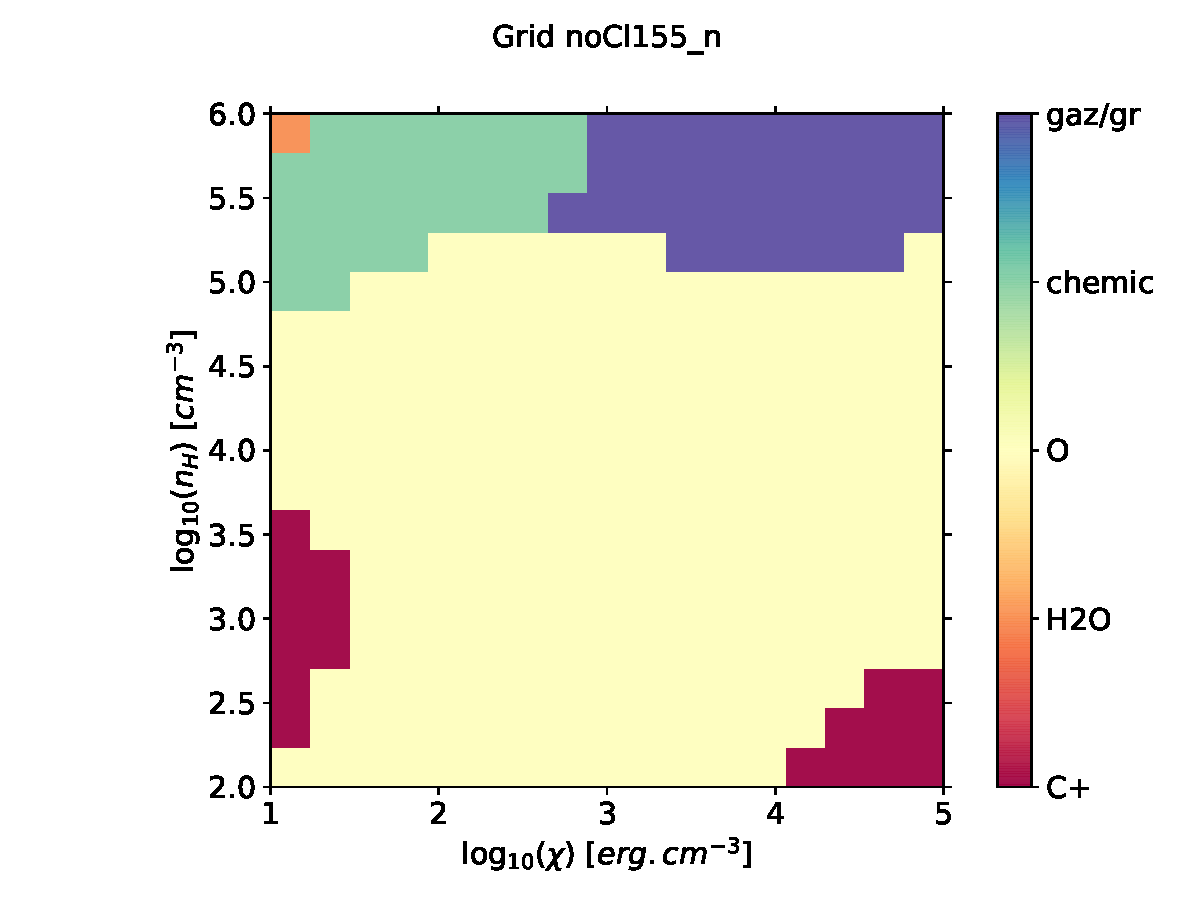
\includegraphics[trim = {0 0 0 1cm },clip,width=1\textwidth]{figure/H2/grid_janev/mapLmax.pdf}
        \caption{Prescription de Janev}
    \end{subfigure}
    ~ 
    \begin{subfigure}[t]{0.49\textwidth}
        \centering 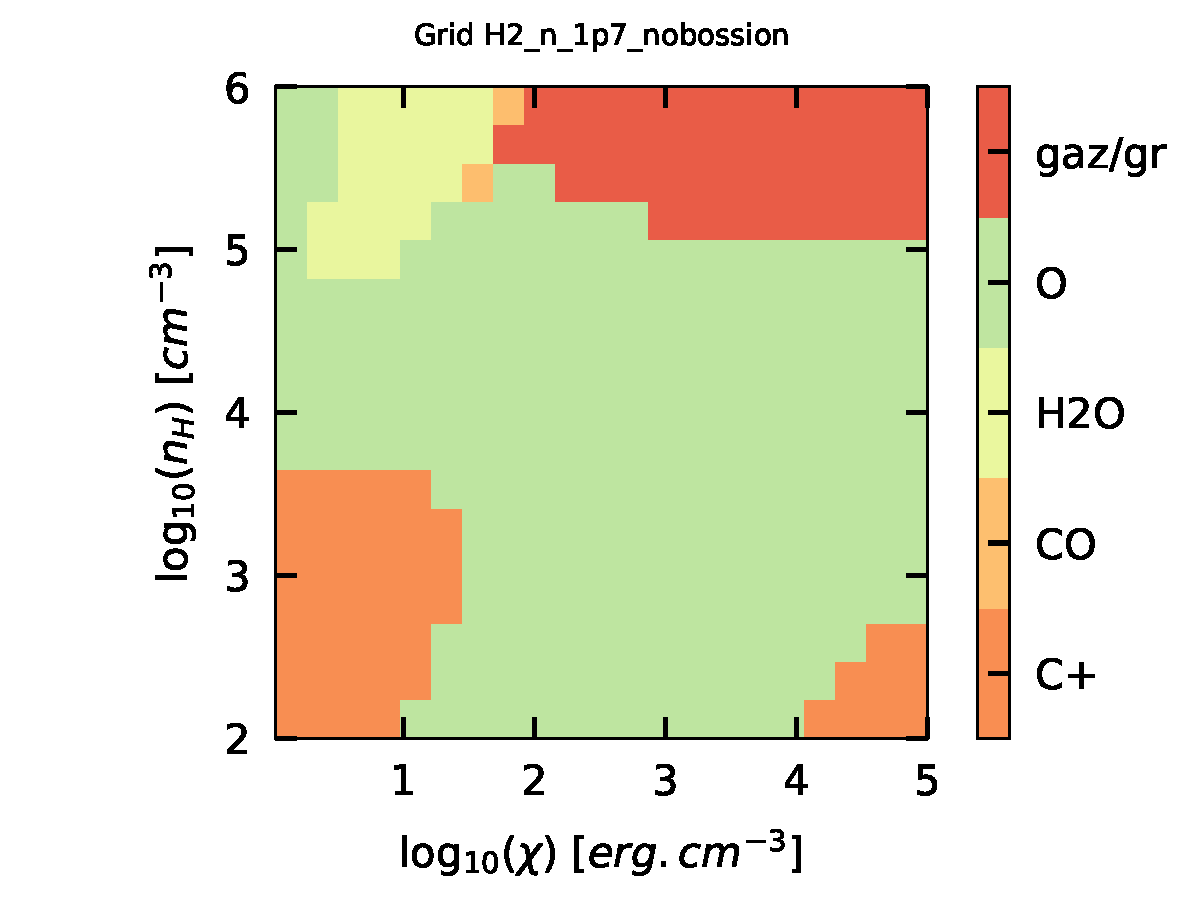
\includegraphics[trim = {0 0 0 1cm },clip,width=1\textwidth]{figure/H2/grid_glover/mapLmax.pdf}
        \caption{Prescription de Glover}
    \end{subfigure}
    \caption{Processus de refroidissement dominant en bord de région atomique}
    \begin{minipage}{\textwidth}
    Les noms "O", "H2O", "CO" et "C+" désignent des processus de refroidissement par émission des espèces $\mathrm{O}$, $\mathrm{H}_2\mathrm{O}$, $\mathrm{CO}$ et $\mathrm{C}^+$ respectivement. "gaz/gr" réfère à la thermalisation du gaz avec les grains du nuage généralement plus froid ($\mathrm{T}\sim20$ K) et "chemic" au bilan thermique des réactions chimiques qui est ici endothermique.
    \end{minipage}
    \label{fig:H2:JanevGlover:Lmax}
\end{figure}


\begin{figure}[!p]  
    \centering
    \begin{subfigure}[t]{0.49\textwidth} % "0.49" donne ici la largeur de l'image
        \centering 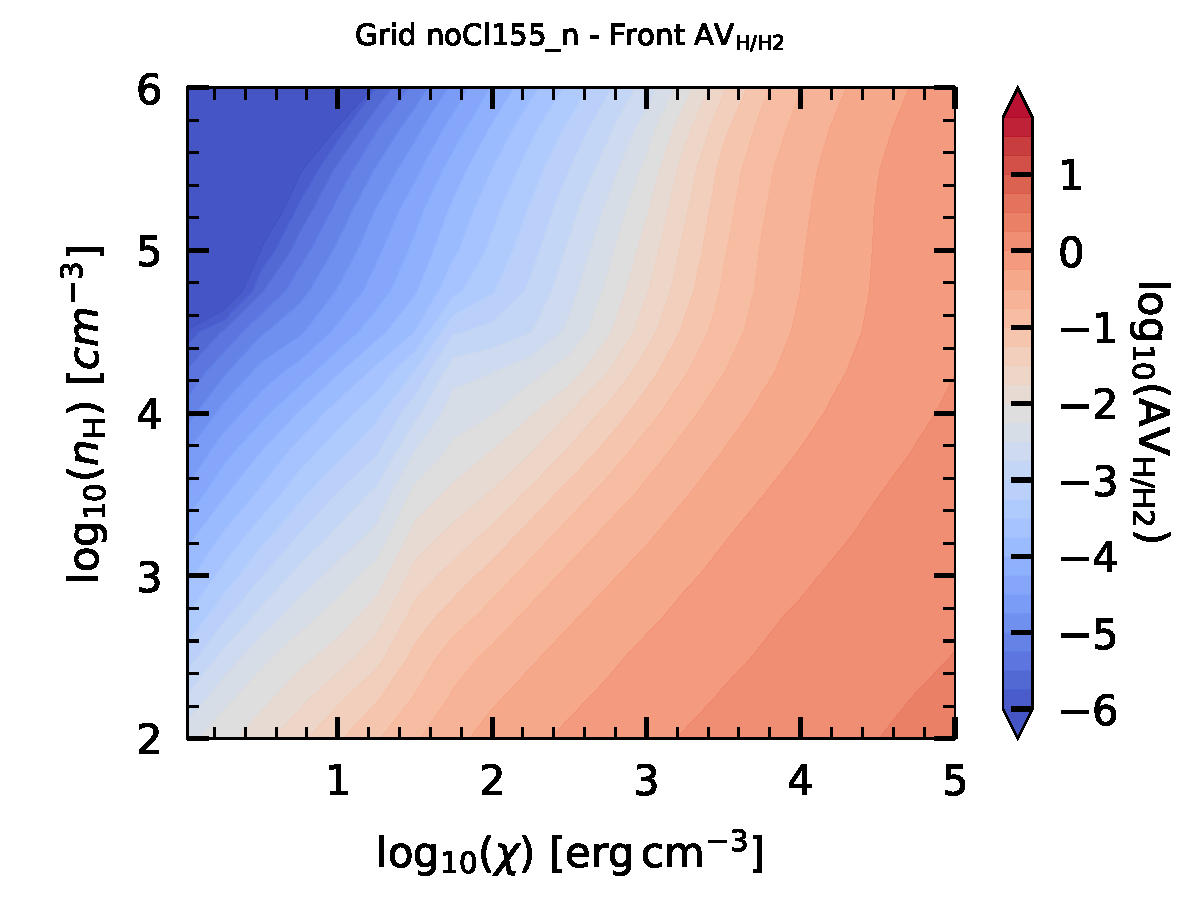
\includegraphics[trim = {0 0 0 1cm },clip,width=1\textwidth]{figure/H2/grid_janev/HH2_AV.pdf}
        \caption{Prescription de Janev}
    \end{subfigure}
    ~ 
    \begin{subfigure}[t]{0.49\textwidth}
        \centering 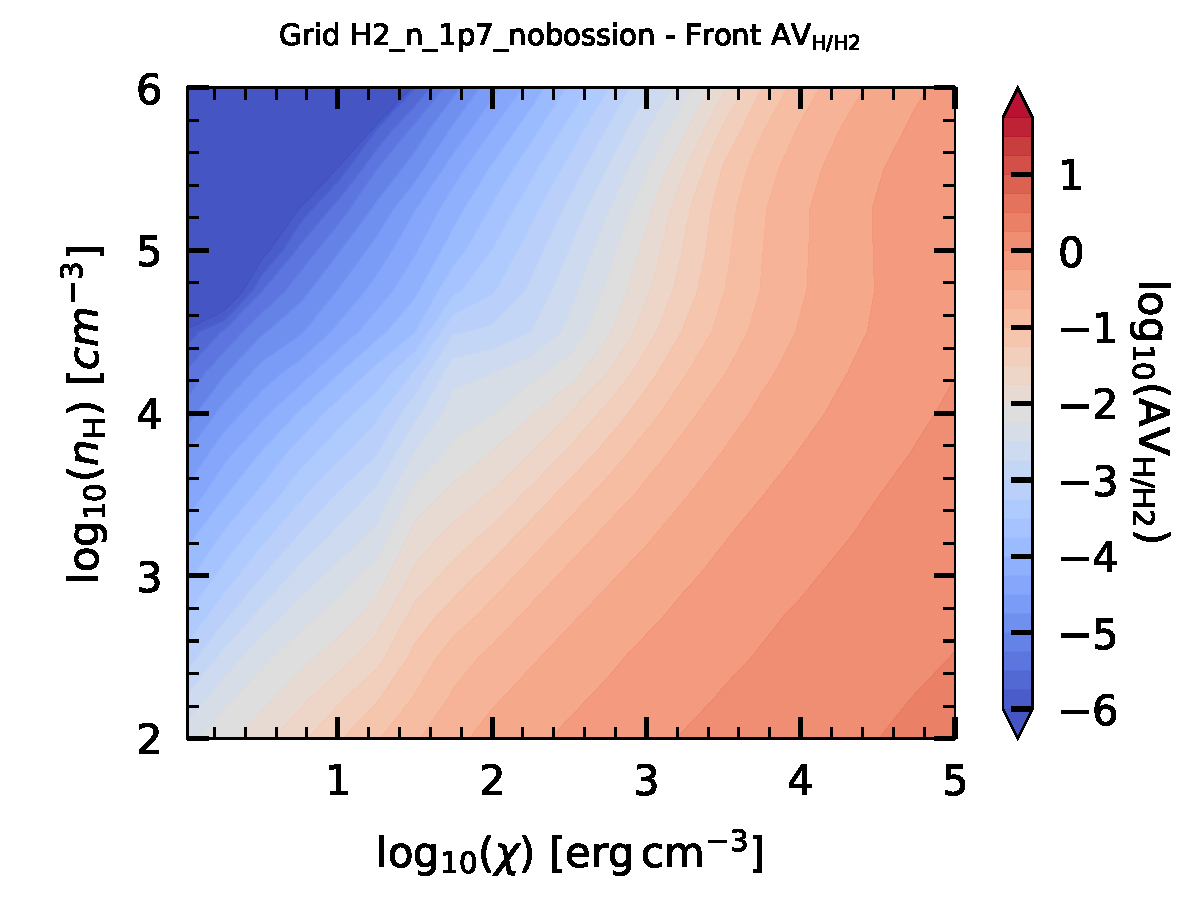
\includegraphics[trim = {0 0 0 1cm },clip,width=1\textwidth]{figure/H2/grid_glover/HH2_AV.pdf}
        \caption{Prescription de Glover}
    \end{subfigure}
    \caption{Comparaison des $\mathrm{A}_\mathrm{v}$ de la transition $\mathrm{H}/\mathrm{H}_2$ des modèles utilisant la prescription de Janev et de Glover}
    \label{fig:H2:JanevGlover:AVHH2}
\end{figure}
 
 \begin{figure}[!p]
    \centering
    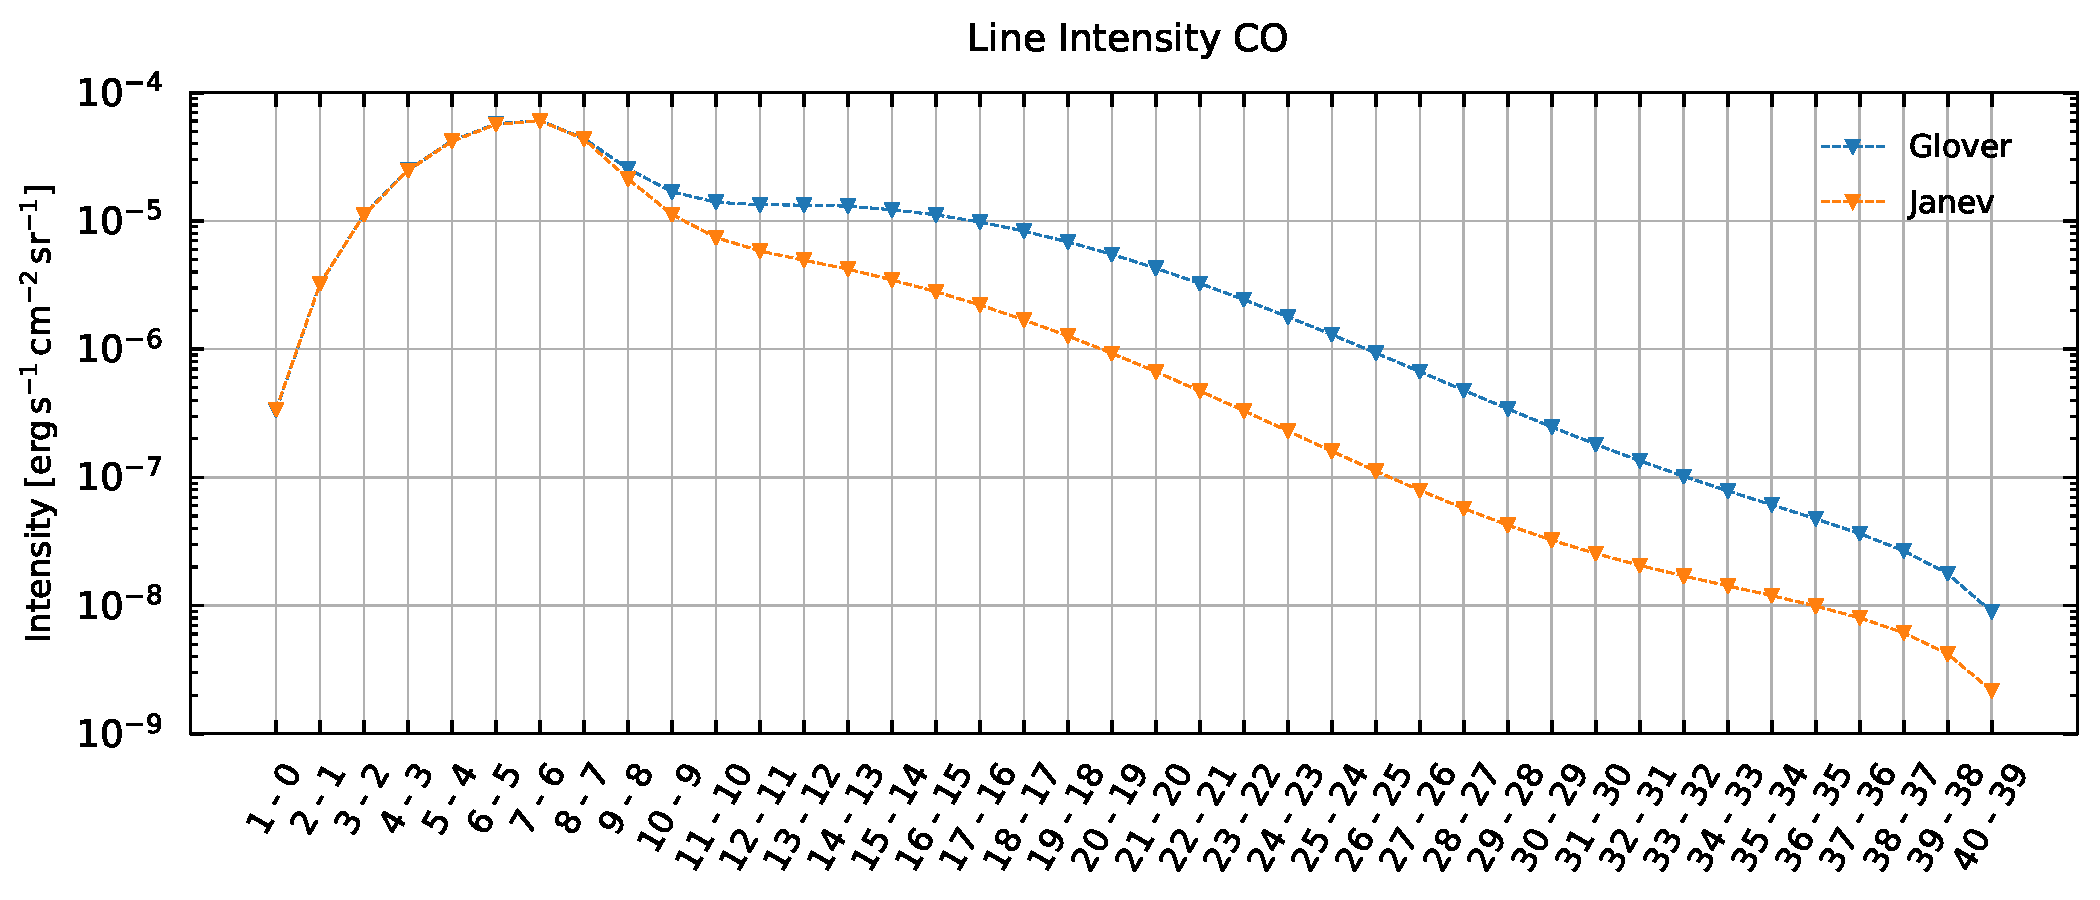
\includegraphics[trim = {0 0 0 1cm },clip,width=1\textwidth]{figure/H2/bosse_dcte_janevVSglover/I_comp_CO.pdf}
    \caption{Raies d'émissions du $\mathrm{CO}$ pour un modèle à densité constante ($n_\mathrm{H} = 10^{5.5}$ et $\chi = 10^4$) utilisant la prescription de Glover ou bien celle de Janev. Les transitions écrites sur l'axe des abscisses signifient les transitions des niveaux rotationnels de la molécule $\mathrm{CO}$.}
    \label{fig:H2:bosse:ICO}
\end{figure}

\end{appendices}
